\chapter{Analysis}
%\textbf{TODO:ROADMAP!!!!!!, which includes sort of a table of contents for the chapter}
This chapter is an extensive discussion on the information and data analysis techniques used to extract the measurement. First we will talk about the building blocks of the measurement and then we will talk about the event plane analysis techniques.
\section{The Building Blocks of the Measurement}
Prior to any analysis, the raw data collected by various PHENIX subsystems must be reconstructed into well-defined software objects encapsulating the physical properties of the particles that traversed the detector. Although we have already discussed the subsystems used in this analysis in chapter III, this section provides in-depth information on central arm tracks, FVTX clusters, and BBC photomultiplier tubes (PMTs), and the physics variables they contain. 

%In this section, I will be detailing the relevant direct observables used in this measurement. They include parameters from central arm tracks, FVTX clusters, and BBC PMTs. Although the Central Arms, FVTX, and BBC have already been described in chapter 3, I will go into more detail into the parameters available and their mathematical precision. 

\begin{figure}[!h]
\begin{center}
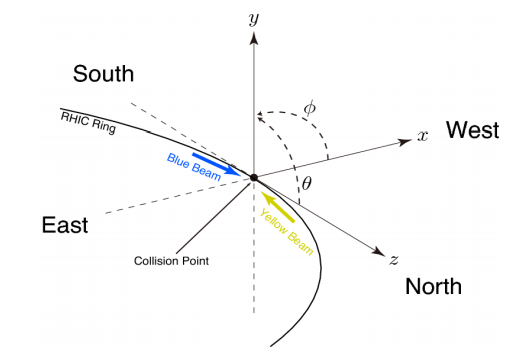
\includegraphics[width=0.55\linewidth]{figs/phenix_coord.png}
\caption{Reference coordinate system for the PHENIX detector. The origin is set at the collision point, around which the detector is centered. The beam runs paralell to the (longitudinal) $z-$axis, where the direction of positive $z$ is defined as \emph{north}. The \emph{east} and \emph{west} directions are defined as perpendicular to the longitudinal direction, where the direction of positive $x$ is defined as west.}
\end{center}
\end{figure}

%\begin{figure}[!h]
%\begin{center}
%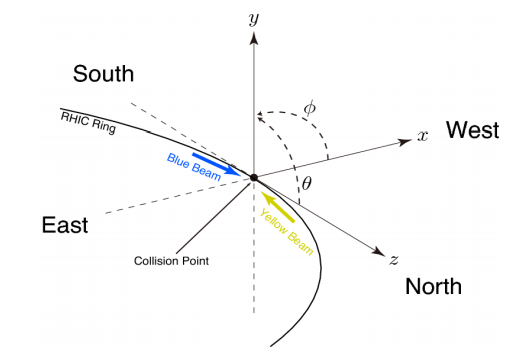
\includegraphics[width=0.55\linewidth]{figs/phenix_coord.png}
%\caption{For reference, I show the PHENIX coordinate system here. The origin is in the middle of the PHENIX detector at the collision %point. North and south are parallel to beam axis. East and west are transverse to the beam axis. Central detectors have a west and an %east arm on either side of the beam. Forward detectors have a north and a south arm relative to the origin.}
%\end{center}
%\end{figure}
%-todo: list all parameters used in the analysis. show some performance plots
\subsection{Central Arm Tracks}
%\textbf{TO DO: ADD A FIGURE CNT}
Central arm (CA) tracks are the representation of charged particles emitted from the heavy ion collision, which are detected by detectors in the PHENIX central arms. There are two central arms, each one covering an acceptance of $\eta < |0.35|$ and $\frac{\pi}{2}$ in pseudorapidity and azimuth, respectively. The relevant detectors for this analysis include the Drift Chamber (DC), the Pad Chambers (PC) and the Ring Imaging Cerenkov (RICH) detector. As previously discussed, the drift chamber provides momentum information; the pad chambers provide track quality metrics; and the RICH provides electron identification. 

The main physical parameter of CA tracks is the momentum vector $\vec{p} = (p_x, p_y, p_z)$ of the particles, defined at the collision vertex. This analysis uses tracks with momentum $0.02 < |p_T| < 3.5$ GeV/$c$, where the momentum resolution is good, as shown in Fig. \ref{fig:dc_mom_res}. The azimuthal angle and pseudorapidity of the track are calculated from the components of its momentum vector, as follows: 
\begin{align}
\phi &= \arctan( \frac{p_y}{p_x} ),\\
\eta &= ArcSinH(\frac{p_z}{p_T}). 
\label{eqn:phi_eta_form}
\end{align}

\begin{figure}[!h]
\begin{center}
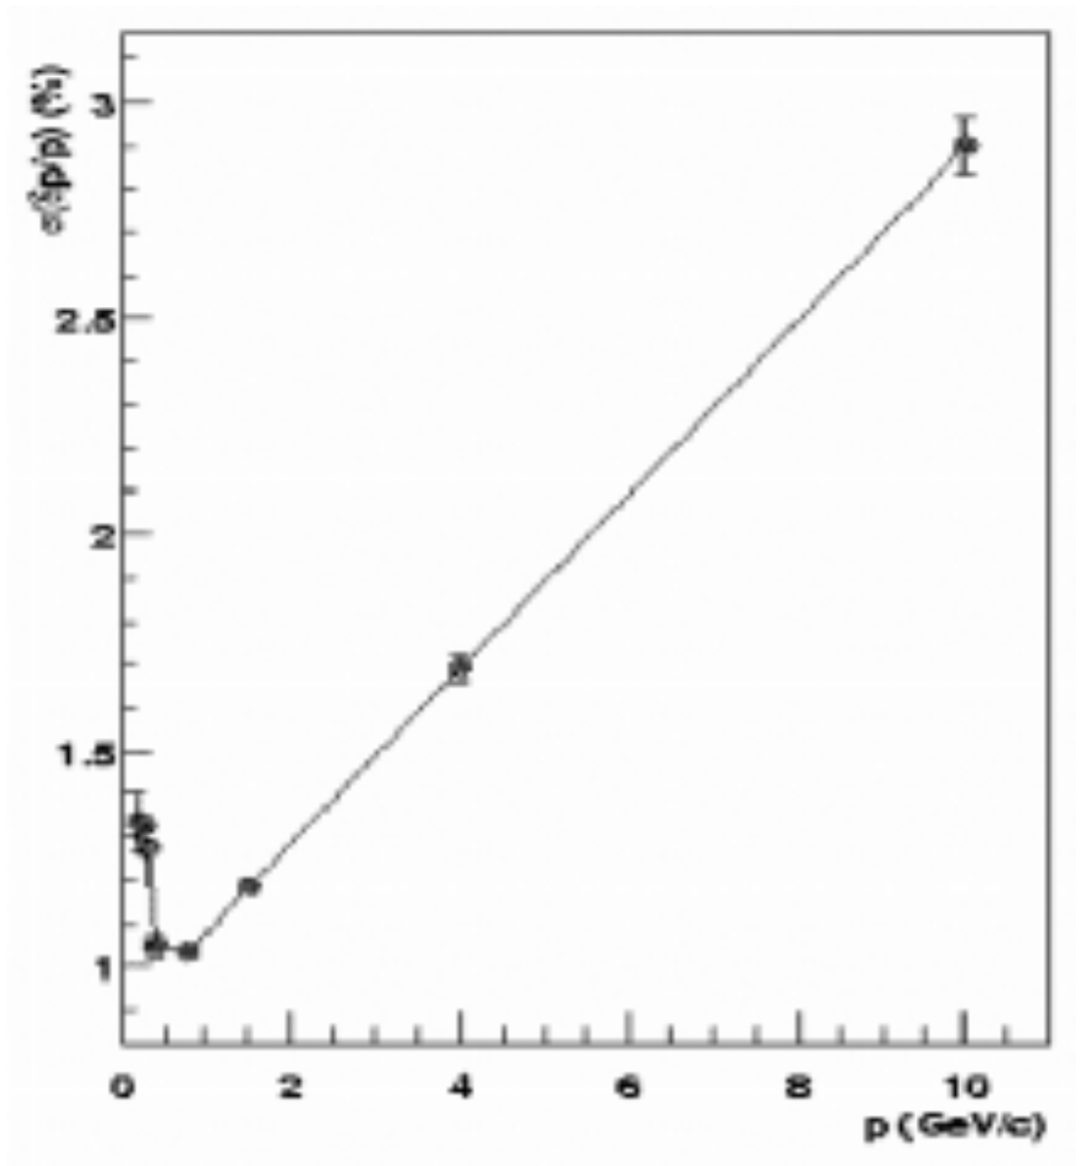
\includegraphics[width=0.45\linewidth]{figs/dc_mom_res.png}
\caption{Momentum resolution $\sigma_{p}/p$ as a function of the reconstructed track momentum, $p$ for simulated single-particle events\cite{CA_spectro}.}
\label{fig:dc_mom_res}
\end{center}
\end{figure}

\begin{figure}[!h]
\begin{center}
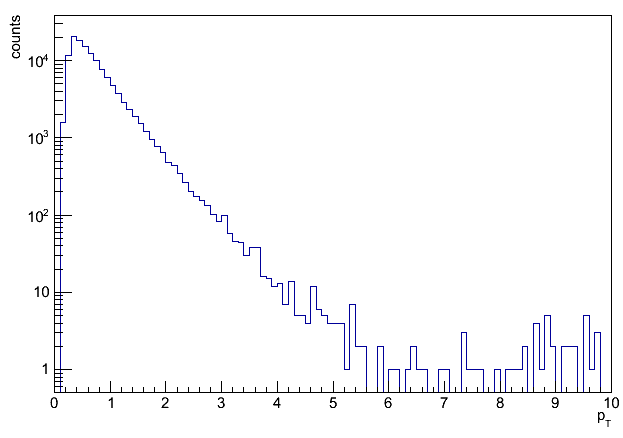
\includegraphics[width=0.45\linewidth]{figs/cnt_pt_dist.png}
\caption{Transverse momentum $p_{T}$ distribution of CA tracks in \pau events at \sqsn = 200 GeV. High $p_T$ tracks observed correspond to unsubtracted background.}
\label{fig:dc_mom_dist_T}
\end{center}
\end{figure}
\begin{figure}[!h]
\begin{center}
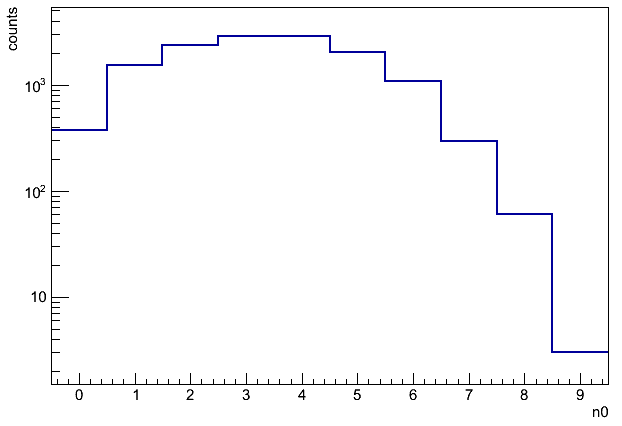
\includegraphics[width=0.45\linewidth]{figs/n0_dist.png}
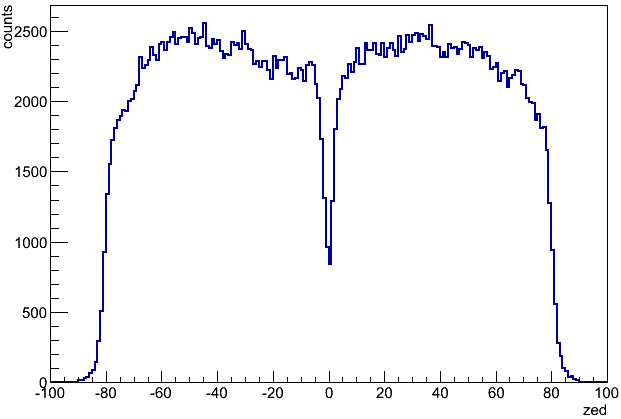
\includegraphics[width=0.45\linewidth]{figs/zed_dist.png}
\caption{The distribution of (left) $n0$, i.e., the number of PMTs fired in the RICH, and (right) $zed$, i.e., the longitudinal position of tracks in the DC, for CA tracks in 0-5\% central \pau events at \sqsn = 200 GeV. The structure observed in the $zed$ distribution corresponds to a gap in the detector acceptance.}
\label{fig:n0_and_zed}
\end{center}
\end{figure}

\begin{table}[h!]
\caption{Quality categorization of CA tracks, as a function of PC1 and DC wire hits. The quality parameters used in this analysis are 31 and 63.}
\begin{center}
%    \begin{tabular}{| l | l | l | | | | | | }
    \begin{tabular}{ccccc}
    \hline
    Quality & PC1 found  & PC1 unique & UV found & UV unique\\ \hline
    17,18,19 & 1 & 0 & 0 & 0\\ \hline
    21,22,23 & 1 & 0 & 1 & 0\\ \hline
    29,30,31 & 1 & 0 & 1 & 1\\ \hline
    49,50,51 & 1 & 1 & 1 & 0\\ \hline
    61,62,63 & 1 & 1 & 1 & 1\\ \hline
    \end{tabular}
\end{center}
\end{table}

\begin{table}[h!]
\caption{Quality categorization of CA tracks, as a function of DC wire momentum information. The quality parameters used in this analysis are 31 and 63.}
\begin{center}
%    \begin{tabular}{| l | l | l | | | | | | }
    \begin{tabular}{ccc}
    \hline
    Quality & X1 used  & X2 used\\ \hline
    17,21,29,49,61 & 1 & 0 \\ \hline
    18,22,30,50,62 & 0 & 1 \\ \hline
    19,23,31,51,63 & 1 & 1 \\ \hline
    \end{tabular}
\end{center}
\end{table}

In addition to momentum, CA tracks provide a number of other parameters that can be used to ensure the quality of tracks and isolate a sample corresponding to charged hadrons. These include $zed$ in the DC, d$\phi$ and d$z$ in the PC, $n0$ in the RICH, and the general track quality calculated from DC and PC information. These variables are defined as follows:

\begin{itemize}
\item The $zed$ variable corresponds to the longitudinal position of the track in the DC, as shown in Fig. \ref{fig:n0_and_zed}
\item The d$phi$ and d$z$ variables quantify the distance between a track projection and its associated hits in the PC. In order to make standard cuts on these variables, their distribution must be calibrated to a standard Gaussian in a procedure known as sigmalization, described in subsection \ref{sec:pc_sigmala}
\item The $n0$ variable, used for electron identification, corresponds to the the number of PMTs fired in the RICH that match the DC track projection, as shown in Fig. \ref{fig:n0_and_zed}
\end{itemize}

\begin{table}[h!]
\caption{Central Arm Track Cuts.}
\begin{center}
    \begin{tabular}{| l | l | l | }
    \hline
    $variable$ & cuts  & units\\ \hline
    $p$ & 0.02 $< p < $ 10.0  & GeV/c\\ \hline
    zed & $|zed| <$75  & cm \\ \hline
    PC3 d$\phi$ & $|d\phi|<$2.0  & radians $\times10^{9}$ \\ \hline
    PC3 dz & $|dz|<$2.0 & cm \\ \hline
    n0 & n0$<=$0 & count \\ \hline
    quality & 63 or 31& N/A \\ \hline
    \end{tabular}
\end{center}
\end{table}

\subsubsection{Sigmalization of PC Variables}
\label{sec:pc_sigmala}
The goal of PC variables d$z$ and d$\phi$ is to provide criteria to determine if the $\phi$ orientation and $z$-direction of the track match between the third layer of the PC and the DC. The sigmalization is done in the minimum bias sample and is valid for all other centrality selections.
We did the sigmalization procedure for tracks in different transverse momentum bins, separately in the east
and west arms, and for positive and negative particles. The d$\phi$ and $d$z distributions
are fitted with a double-Gaussian function and then the parameters are smoothed as
a function of $p_T$ . Fig. \ref{fig:pc3_sig} a) shows a fit to the sigmalized
d$\phi$ distribution and Fig. \ref{fig:pc3_sig} b) shows a fit to the sigmalized d$z$ distribution for tracks with 1.0 $< p_T <$ 1.1 (GeV/c)
in both west and east arms as well as both positively and negatively charged particles.
Then we fit the signal Gaussian mean and sigma by some polynomial functions.  Once these variables have been sigmalized, we select only
the tracks within a 2$\sigma$ cut.

\begin{figure}[h!]
\begin{center}
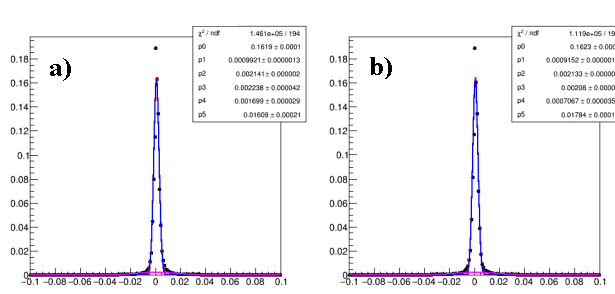
\includegraphics[scale=0.45]{figs/pc3dphi.png}
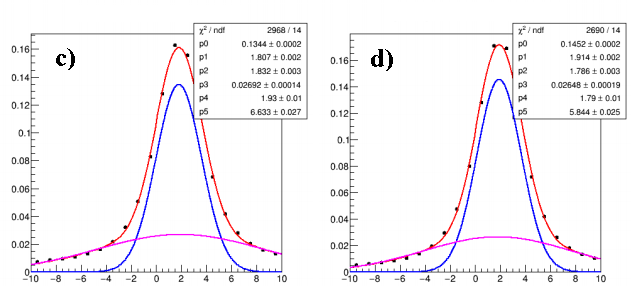
\includegraphics[scale=0.45]{figs/pc3dz.png}
\end{center}
\label{fig:pc3_sig}
\caption{The top plots show the PC3 matching d$\phi$ fit in range 1.0 $< pT <$ 1.1 (GeV/c).
The blue and pink lines are single Gaussian fits to the signal and background, respectively, which are combined in the red line.
The bottom plots show the result of the d$z$ sigmalization, done in the same was as for d$\phi$.}
\end{figure}

%\subsection{Central Arm Tracking}

%In p+Au collisions, the average number of reconstructed CNT (before cuts) is (\textbf{TO DO: QUANTIFY THIS}).
\subsection{FVTX Clusters}
The FVTX consists of four silicon layers in the north and south directions, covering an acceptance of $1 < | \eta | < 3$ and spanning the full azimuth. FVTX clusters correspond to the spatial location where charged particles hit one of the silicon layers. Each cluster is expected to correspond to a single charged particle in the case of \pau collisions, because of the low multiplicity relative to Au+Au collisions. These clusters have a spatial resolution in $x$ and $y$ of 50 $\mu$m, and have an RMS along the $z$-direction that coresponds to the width of an FVTX layer, of $\frac{200}{\sqrt{12}}$ $\mu$m \cite{Aidala201444}. Due to the \pau collision system's inherent asymmetry, the majority of particles are produced in Au-going (i.e., south) direction. Taking into account this asymmetry, only the clusters from the south arm are used for calculations in this analysis. In a typical 0-5$\%$ centrality event, there are on average ~1500 FVTX clusters in the south arm alone.

%%check numbers in this section
\begin{figure}[!h]
\begin{center}
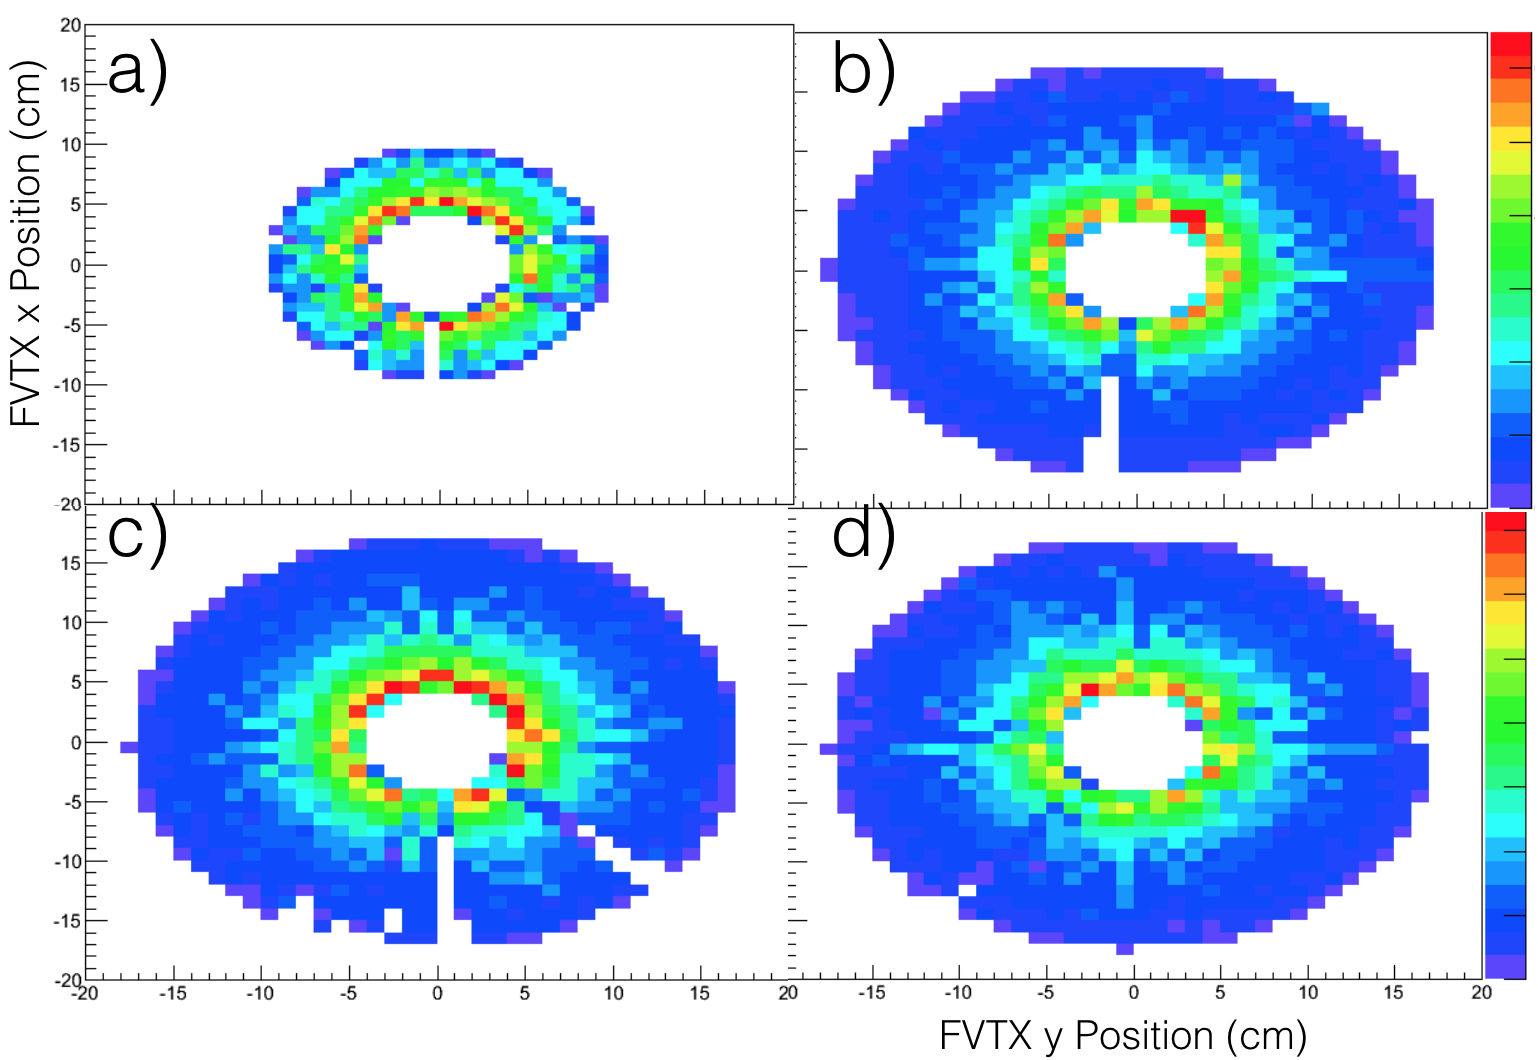
\includegraphics[width=0.55\linewidth]{figs/fvtx_clus_xy.png}
\caption{Distribution of FVTX clusters in $x$ and $y$ for layers 1, 2, 3, and 4 for panels a), b), c), and d), respectively. The color scale corresponds to the number of counts.}
\label{fig:dc_mom_res}
\end{center}
\end{figure}

\subsection{BBC PMTs}
The BBC provides information on the position, time of arrival, and number of charged particles that hit the BBC's quartz radiator material. The BBC acceptance is $3.1 < |\eta| < 3.9$ and spans the full azimuth. The resolution of the detector in $x$ and $y$ is 5 cm, corresponding to the diameter of a BBC PMT. Like with the FVTX, the $z$ resolution is simply the width of the active area of the BBC divided by $\sqrt{12}$. In addition to spatial information, the BBC provides charge information, calibrated so that a value of 1.0 corresponds to a single charged particle hitting the detector. Fig \ref{fig:bbc_rings} shows the layout of the PMTs for the BBC. As discussed in section \ref{sec:bbc_det_sec}, the information regarding arrival time and particle charge can be used to calculate the $z$-vertex of the collision. 
\begin{figure}[h!]
\begin{center}
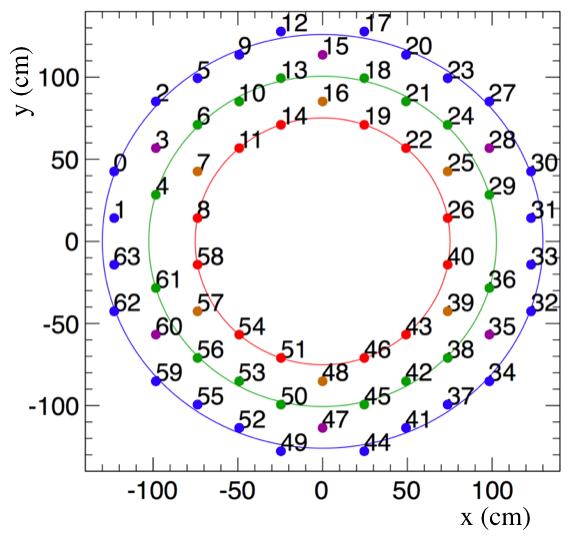
\includegraphics[width=0.55\linewidth]{figs/bbc_rings.png}
\caption{Diagram showing the positions of the PMTs for the BBC-south detector. Rings shown with the same color indicate PMTs at an approximate common radius.}
\label{fig:bbc_rings}
\end{center}
\end{figure}

%\section{Two-particles Correlation}
%\subsection{Measurement in p+p and p+Au}


\section{The Event Plane Method}
\textbf{TODO: We want to measure v2, which is related to collective behavior as evidence by correlations among particles. These correlations exist relative to orientation of the collision. The event plane method measures ... from final state particles...}
The event plane method uses final-state particles to calculate the event plane angle from the data. A different event plane angle is defined for each harmonic, and is denoted as $\Psi_n$ where $n$ is the harmonic number. The definition for $\Psi_n$ is related to the calculation of the Q-vector:

For an event with $N$ particles, define the flow vector $\vec{Q}$ as follows:

\begin{align}
Q_x &= \sum_i^{N}( w_i * \cos(n * \phi_i)) \\
Q_y &= \sum_i^{N}( w_i * \sin(n * \phi_i)) \\
Q_w &= \sum_i^{N}( w_i )
%\Psi_n &= \arctan( \frac{Q_y}{Q_x} ),
\label{eqn:general_ep_math}
\end{align}

where $i$ is the $i$th particle in the event, $\phi_i$ is the azimuthal angle of the particle, $w_i$ is the weight factor, and $n$ is the harmonic number.

We define the $n$th order event plane as
$$\Psi_n = \arctan \left( \frac{Q_y}{Q_x} \right) $$

Once the event plane has been calculated, the flow harmonics ($v_n$) are defined as
\begin{equation}
v_n = \frac{\langle \langle\cos(n(\phi - \Psi_n))\rangle \rangle}{Resolution(\Psi_n)},
\end{equation}

\textbf{TODO: Make distinction, event plane and Q are defined at the event level, but v2 is defined over many events}

where $\langle \langle \rangle \rangle$ indicates that $\cos(2\phi-\psi)$ is averaged over all particles in the same event, and the resulting $v_2$ must be averaged over many events \cite{PhysRevC.58.1671}. 

As discussed in section xxx, [WHY IS THERE A RESOL CORRECTION? what does it correct for? How is it calculated?]. The resolution of $\Psi_n$ is calculated using the 3-subevent method. It is important to note the the set of particles used to calculate $\Psi_n$ and $\phi$ must be different in order to avoid
autocorrelations. This is usually done by imposing an $\eta$ gap between to two particle sets.

\textbf{TODO: Maybe remove this redundant definition of the event plane. State it in words.}

For this analysis, the event plane is calculated separately for each of the forward detectors mentioned above, i.e., the BBC and the FVTX. [Say how detector elements are used to compute phi, and what the weights are.]


For the FVTX, the Q-vector is calculated in each event as
\begin{align}
Q_x &= \sum^{NClus}_i( \cos(n * \phi_i)) \\
Q_y &= \sum^{NClus}_i( \sin(n * \phi_i)) \\
\phi_i &= \arctan(\frac{Clus_{y}^i}{Clus_{x}^i})
\end{align}
where NClus is the number FVTX clusters in that event and $Clus_{y,x}^i$ are the $x$ and $y$ components of the $i$th FVTX Cluster in that event. This Q-vector is calculated with no cluster dependent weight factor as each cluster is taken to be equal weight.
(since no charge information is available in the FVTX). 

For the BBC, the Q-vector is calculated in each event as
\begin{align}
Q_x &= \sum^{NPMT}_i( w_i \cos(n * \phi_i)) \\
Q_y &= \sum^{NPMT}_i( w_i \sin(n * \phi_i)) \\
Q_w &= \sum^{NPMT}_i( w_i ) \\
\phi_i &= \arctan(\frac{PMT_{y}^i}{PMT_{x}^i}) 
\label{eqn:bbc_ep_eqns}
\end{align}
where $w_i$ is the charge collected on the PMT and NPMT is the number of PMTs that fired (above threshold) in each event.

Finally, the $v_n$ are calculated using a combination of the BBC or FVTX Q-vectors and the CA tracks as
\begin{equation}
v_n = \frac{\left<\left<\cos(n(\phi^{CA} - \Psi^{BBC,FVTX}_n))\right>\right>}{Resolution(\Psi^{BBC,FVTX}_n)}.
\end{equation}
In this analysis, we are concerned only with measuring the second-order harmonic $v_2$, because it is the easiest harmonic 
\begin{enumerate}
	\item{The second harmonic is usually the largest and easiest to measure harmonic.}
	\item{The second harmonic is physically interesting because it is thought to correspond with flow, along with others.}
\end{enumerate}
\subsection{Event Plane Flattening Calibration}
In order for the event plane to be useful in making a $v_n$ measurement, the event plane angle must be calibrated such that its distribution is uniform. For the event plane method, a physical assumption is made that the true
distribution of $\Psi_n$ angles will be uniform. In other words, there is no preferred event plane angle in heavy ion collision. If the measured $\Psi_n$ distribution is not flat, we attribute that behavior to variations in the efficiency of detecting charged particles as a function of $\phi$. Thus, the event plane calibration procedure seeks to correct for these non-uniformities in acceptance, and restore the $\Psi_n$ distribution to the physical expectation of uniformity.


We employ a procedure to re-center and flatten the measured non-uniform $\Psi_n$ distribution, such as the one shown in Fig.xxx 
%\begin{figure}[htbp]
%\begin{center}
%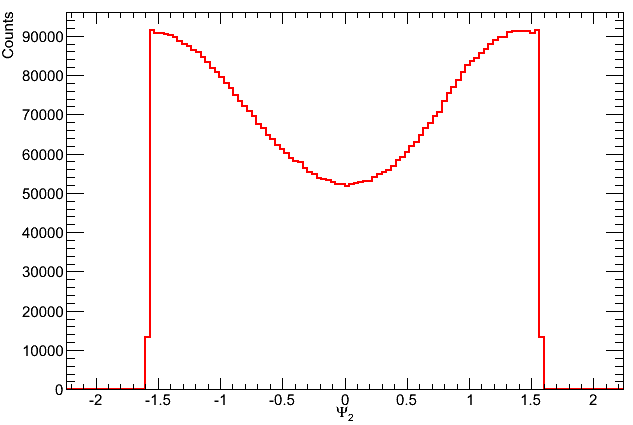
\includegraphics[width=0.65\linewidth]{figs/example_raw_psi2.png}
%\caption{This is the BBC-S $\Psi_2$ distribution before any calibration. The range of the $\Psi_2$ resolution is from $\frac{-\pi}{2}$ to $\frac{\pi}{2}$ because of the periodicity. 
%The raw distribution has a sinusoidal shape.}
%\end{center}
%\label{fig:raw_psi}
%\end{figure}
The red curve in Fig. ~\ref{fig:calibrated_psi} depicts a significant deviation from uniformity in the $\Psi_2$ distribution. The flattening calibration attempts to correct for this 
lack of uniformity by systematically shifting the $\Psi_2$ value of each individual event by an amount corresponding to the deviation of the overall distribution for all events. Although this procedure results in a uniform $\Psi_2$ distribution, applying too large of a correction arising from an exceedingly distorted initial distribution can lead to systematic effects on the $v_2$ measurement, as will be discussed later. Therefore, it is important to address any systematic effects that 

\textbf{TODO:REWRITE!!!!}

In general, the $\Psi_2$ distribution will be non-uniform. However, Thus, it is in the analyzer's best interest
to provide the flattest possible $\Psi_2$ distribution before performing the flattening calibration.
\begin{figure}[!h]
\begin{center}
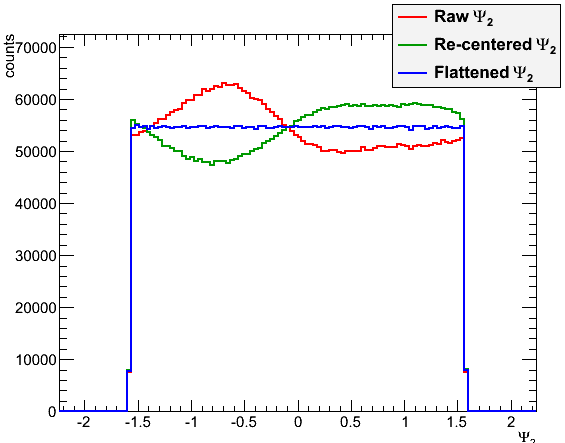
\includegraphics[width=0.65\linewidth]{figs/flattened_example_fvtx.png}
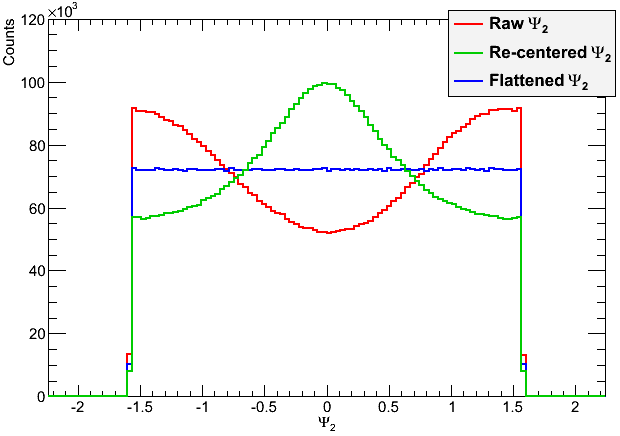
\includegraphics[width=0.62\linewidth]{figs/flattened_example_bbc.png}
\caption{This is the $\Psi_2$ distribution projected over all z-vertex bins at different steps during the calibration. The top is from the FVTX south and the bottom is from the BBC south. The range of the $\Psi_2$ resolution is from -$\frac{\pi}{2}$ to $\frac{\pi}{2}$ because of the periodicity. 
The raw (in red) $\Psi_2$ distribution has a sinusoidal shape. The re-centered (in green) $\Psi_2$ distribution moves the peak and has a width. The flattened (in blue) 
$\Psi_2$ distribution spread out the counts so that there is uniformity. Each calibration step preserves the integral.}
\end{center}
\label{fig:calibrated_psi}
\end{figure}

The flattening calibration requires two steps to completely flatten the $\Psi_n$ distribution. The first step of the calibration is to re-center the peak of the raw $\Psi_n$ distribution to be at 
0.0 radians and to resize the width of the peak. The second step is to Fourier transform the re-centered distribution and use the transformation to shift the $\Psi_n$ values to a uniform distribution. With flattening, each $\Psi_n$ is transformed to $\Psi_n + \Delta\Psi_n$. $\Delta\Psi_n$ is defined as
\begin{equation}
\Delta\Psi_n = \sum^{N}_{i=1}\left(\frac{2}{i}\left(\sin(i \Psi)F^{\cos}_{i}(f(\Psi_n))-\cos(i \Psi)F^{\sin}_{i}(f(\Psi_n)\right)\right),
\label{eq:deltapsi}
\end{equation}
where $N$ is the number of components, $F^{\cos}_{i}(f(x))$ is the $i$th component of the cosine Fourier transform of $f(x)$, and $f(\Psi_n)$ is the $\Psi_n$ distribution.

For this analysis, $N=$12 is a sufficient number of components to flatten the $\Psi_n$ distribution. The re-centering and flattening calibration is done in separate 30 z-vertex bins.

\subsection{Event Plane Resolution Calculation}
As mentioned above, the event plane resolution is calculated using the standard 3-sub event method\cite{PhysRevC.58.1671}. The strategy of this method is to measure $\Psi_n$ with three
different detectors in the same event, in order to better constrain the overall measurement of $\Psi_n$. The event plane resolution is defined as
\begin{equation}
Res(\Psi_n^A) = \sqrt{\frac{\left<\cos(n(\Psi_n^A - \Psi_n^B))\right>\left<\cos(n(\Psi_n^A - \Psi_n^C))\right>}{\left<\cos(n(\Psi_n^B - \Psi_n^C))\right>}},
\label{eqn:res}
\end{equation}
where A,B, and C are three detectors measuring the same event. In this context, the term ``sub-event'' refers to the specific subset of particles measured by a given detector, assuming no decorrelation \cite{PhysRevC.58.1671}. \textbf{TODO: Deal with decorrelation}

\begin{figure}[!h]
\begin{center}
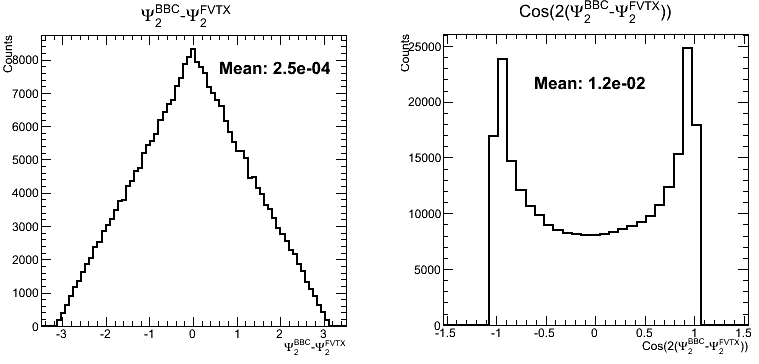
\includegraphics[width=0.85\linewidth]{figs/resolution_intermediate_calc.png}
\caption{Intermediate steps involved in calculating the event resolution. (left) Raw difference between the event planes angles for two different detectors. \textbf{Discuss why it's a triangle...} (right)  The cosine of two times the difference between the two event plane angles. The average of this distribution is used in equation \ref{eqn:res}.}
\label{fig:fvtx_ew_default}
\end{center}
\end{figure}

In this analysis, the three detectors used to provide the required three subevents are the FVTX-south, the BBC-south, and the CA, which span pseudorapidity acceptances of $-3 <\eta < -1$, $-3.9 < \eta < 3.1$, and $|\eta| < 0.35$, respectively. 
Unlike the BBCS and the FVTXS, the CNT detector does not have full azimuthal acceptance coverage. Therefore, the event plane angle cannot be reliably calculated with this detector for events whose event plane points outside of the acceptance. In order to solve this problem, we calculate the event plane resolution using a different, yet mathematically equivalent formulation that does not make use of $\psi_CNT$, as given below:

%However, due to the fact that the CNT detector does not have full azimuthal coverage, the CNT event plane is not well defined for a class of events where the event plane doesn't point into the CNT acceptance, therefore the event plane resolution is calculated via a modified yet mathematically equivalent definition to the one mentioned above. This modified method allows the resolution of the FVTX-S and the BBC-S to be calculated using the CNT without having to calculate CNT event plane. It is defined as
\begin{equation}
Res(\Psi_n^A) = \sqrt{\frac{\left<\left<\cos(n(\Psi_n^A - \phi^{CNT}))\right>\right>\left<\cos(n(\Psi_n^A - \Psi_n^C))\right>}{\left<\left<\cos(n(\phi^{CNT} - \Psi_n^C))\right>\right>}},
\end{equation}
where there is a double average over each CNT track and each event.
%(\textbf{TO DO: Make a Table of Default Event Plane Resolutions})
\begin{table}[h!]
\caption{}
\begin{center}
    \begin{tabular}{| l | l | l | l |}
    \hline
    Detector & $n=2$ & $n=3$  \\ \hline
    FVTXs & 0.216 & 0.010 \\ \hline
    BBCs & 0.052 & 0.010  \\ \hline
%    Wednesday & 10C & 21C & ... \\
    \end{tabular}
\end{center}
\end{table}

\section{Correcting for the Effects of Beam Alignment}
\textbf{REWRITE: Check order}
\begin{figure}[!h]
\begin{center}
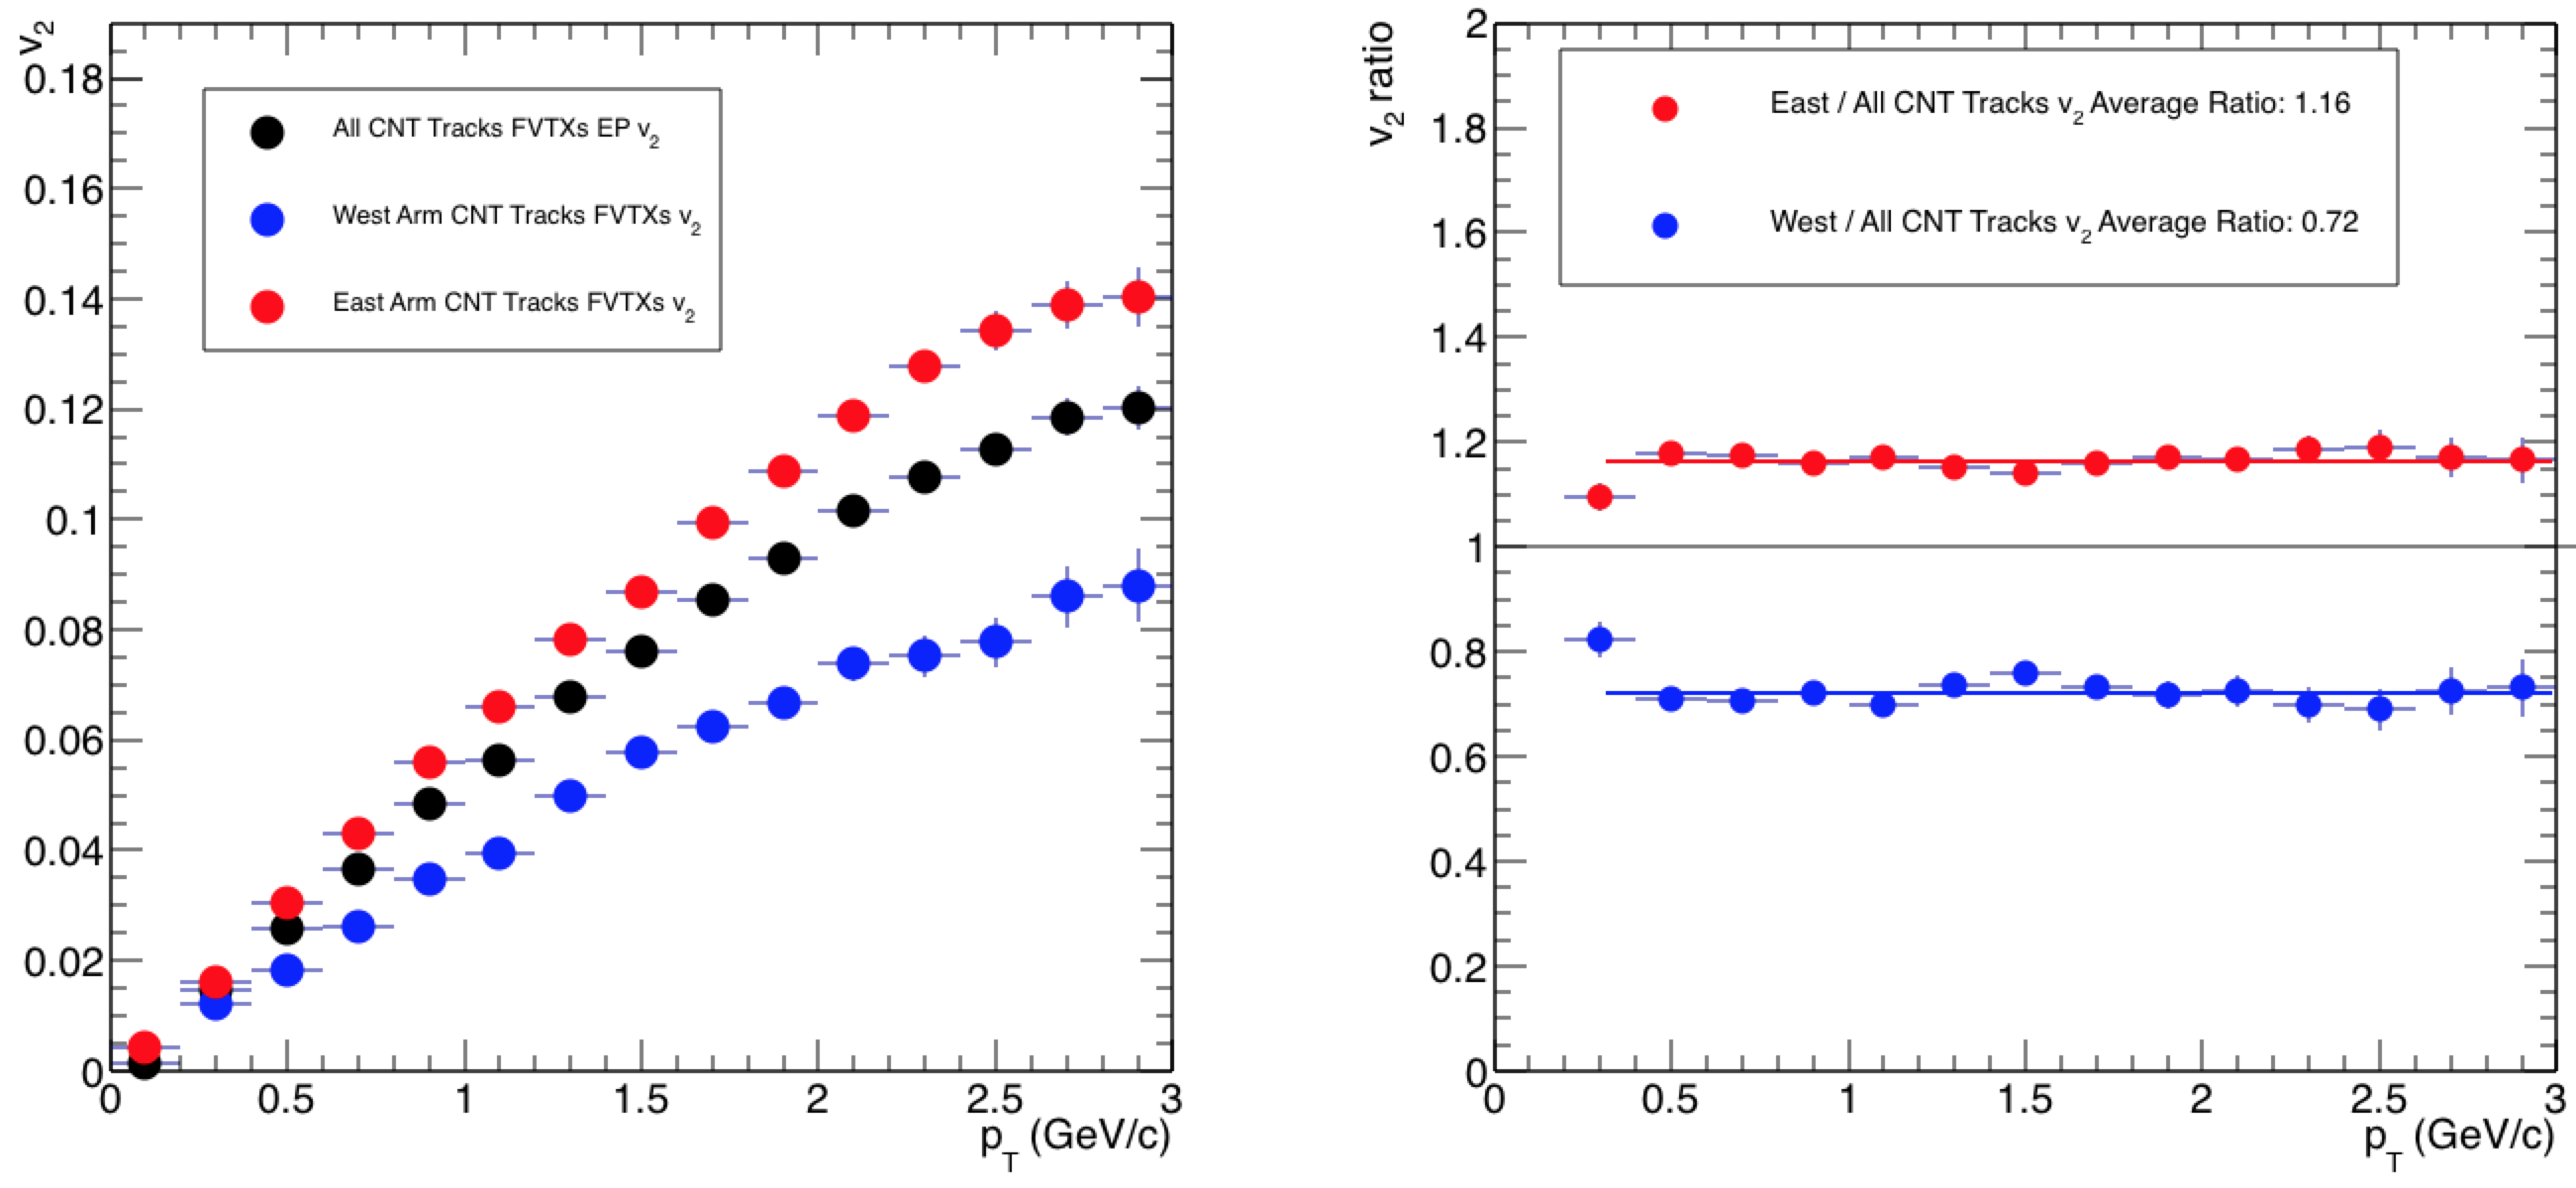
\includegraphics[width=0.85\linewidth]{figs/fvtxs_default_ew.png}
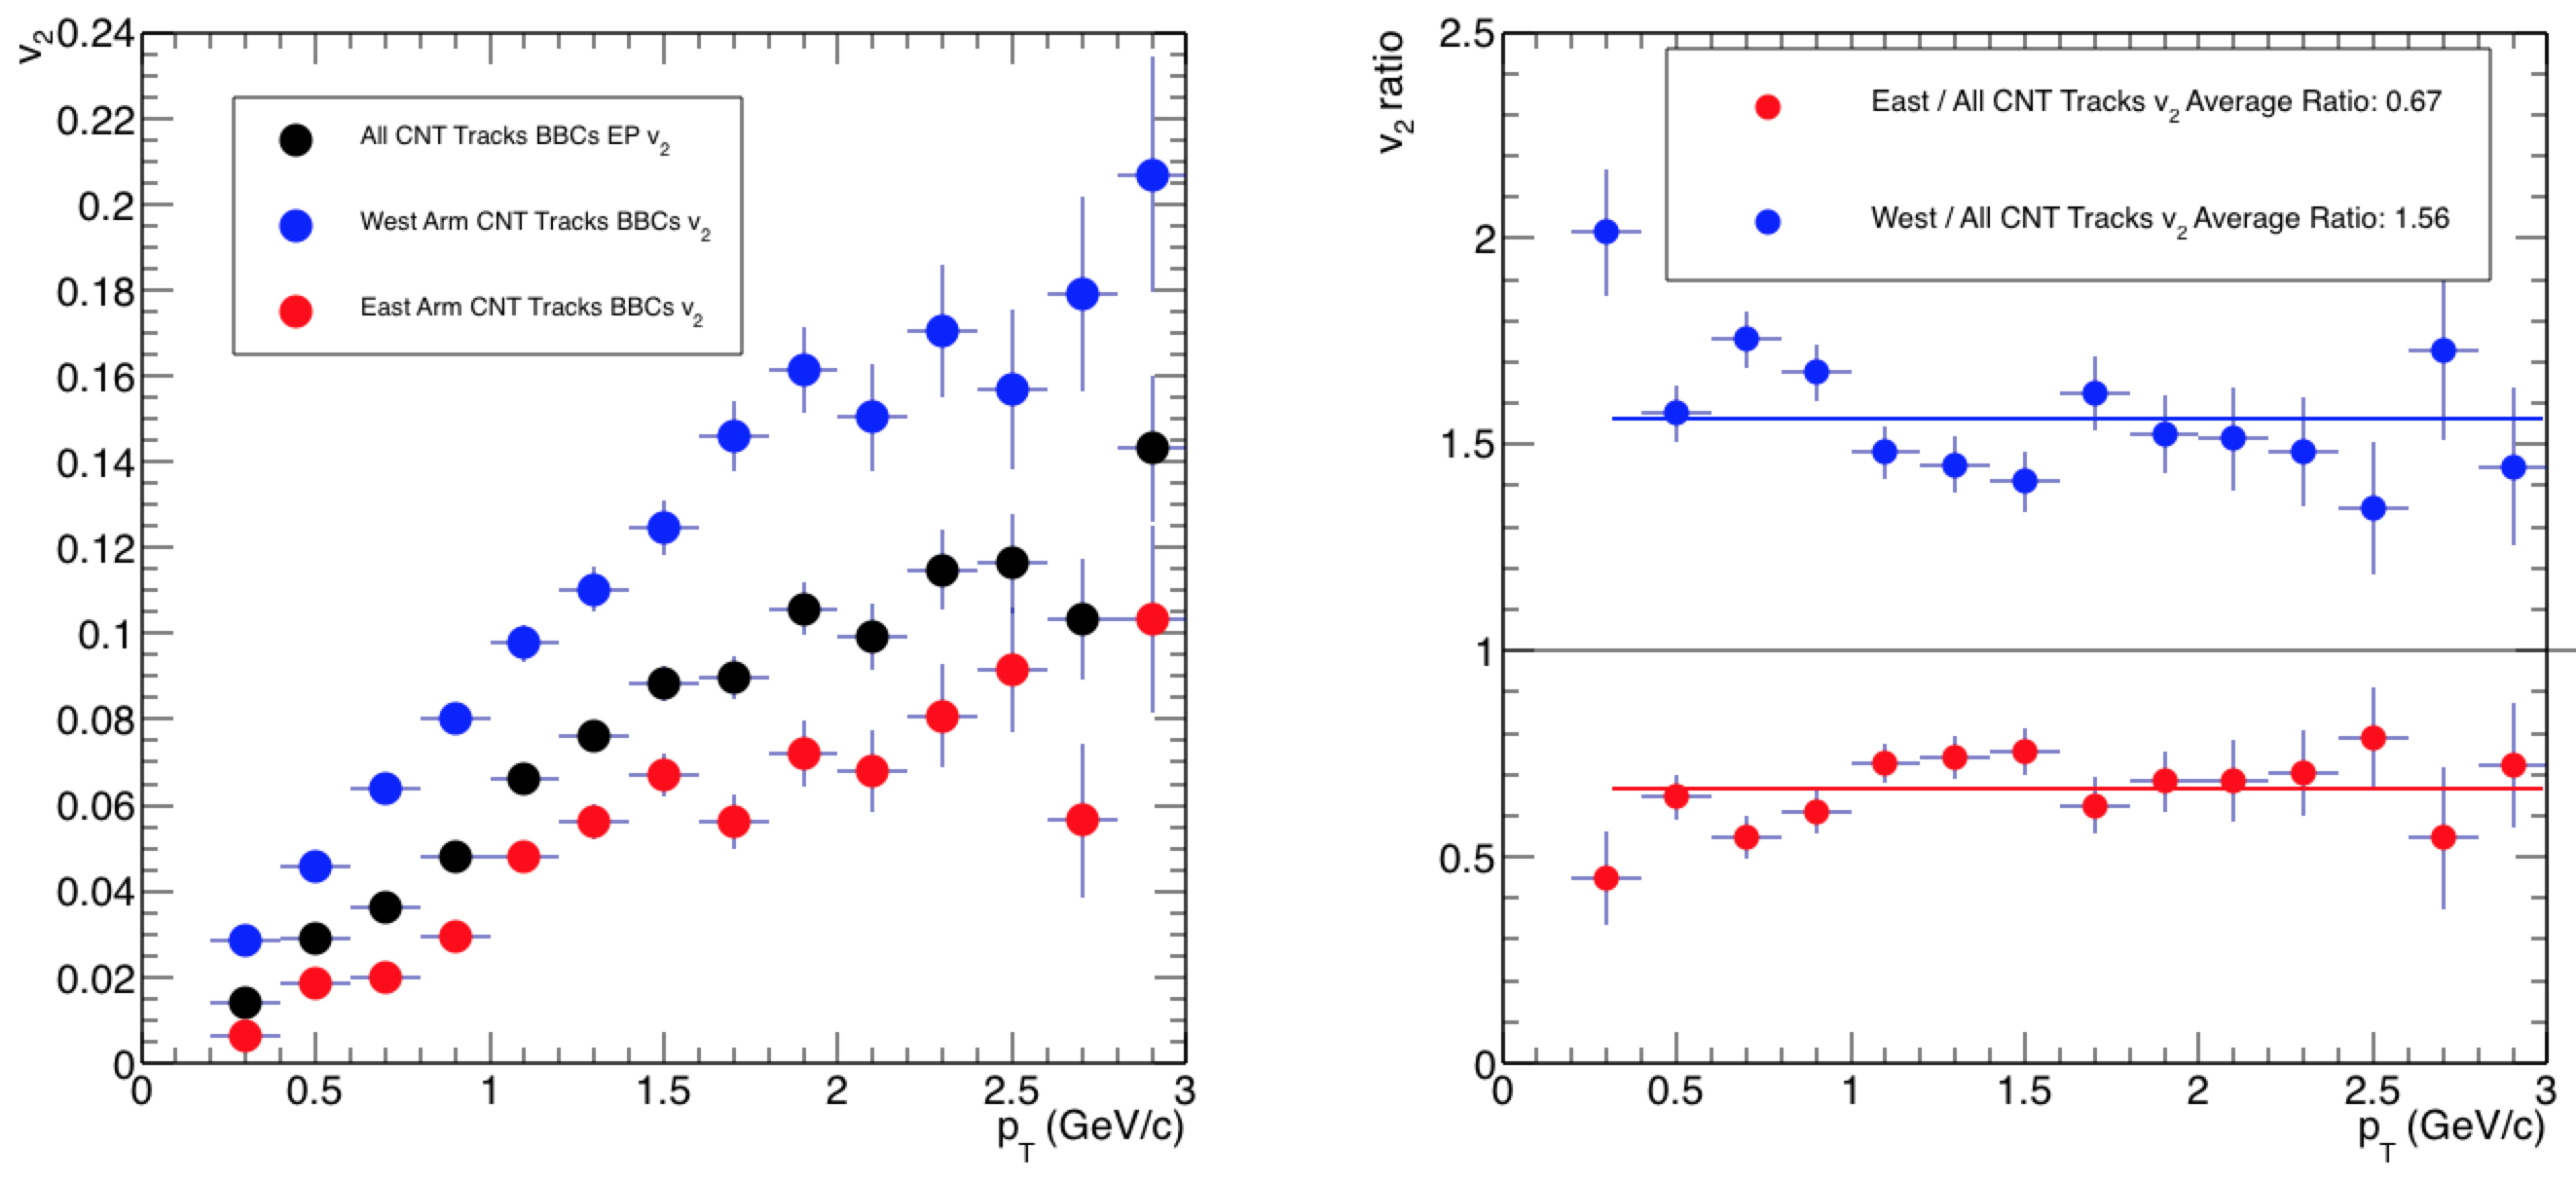
\includegraphics[width=0.85\linewidth]{figs/bbcs_default_ew.png}
\caption{First attempt at measuring $v_{2} (p_T)$ with the event plane as calculated with the FVTXs (top left) and the BBCs (bottom left) in the p+Au @ 200 GeV dataset, using the default resolution as shown in table TBA. The black points show $v_2$ measured using all CNT tracks. The blue and red points show $v_2$ measured using only tracks in the west and east arms, respectively. It is apparent that there is a significant difference depending on which detector arm is used calculate $v_2$. This implies there are systematic errors influencing the measurement. The panels on the right quantify the difference between $v_2$ in the two arms by plotting their ratio to the measurement with inclusive tracks. The ratios are fit with a constant, whose value if shown in the legend.}
\label{fig:fvtx_ew_default}
\end{center}
\end{figure}

As shown in Fig \ref{fig:fvtx_ew_default}, $v_2$ is different when measured using tracks in the west (-1 $<$ $\phi$ $<$ 1 ) and east arm ( 2 $<$ $\phi$ $<$ 4 ) of the CA. This is a systematic effect explained by the colliding beams not being parallel to the longitudinal axis of PHENIX. 

\begin{figure}[h!]
\begin{center}
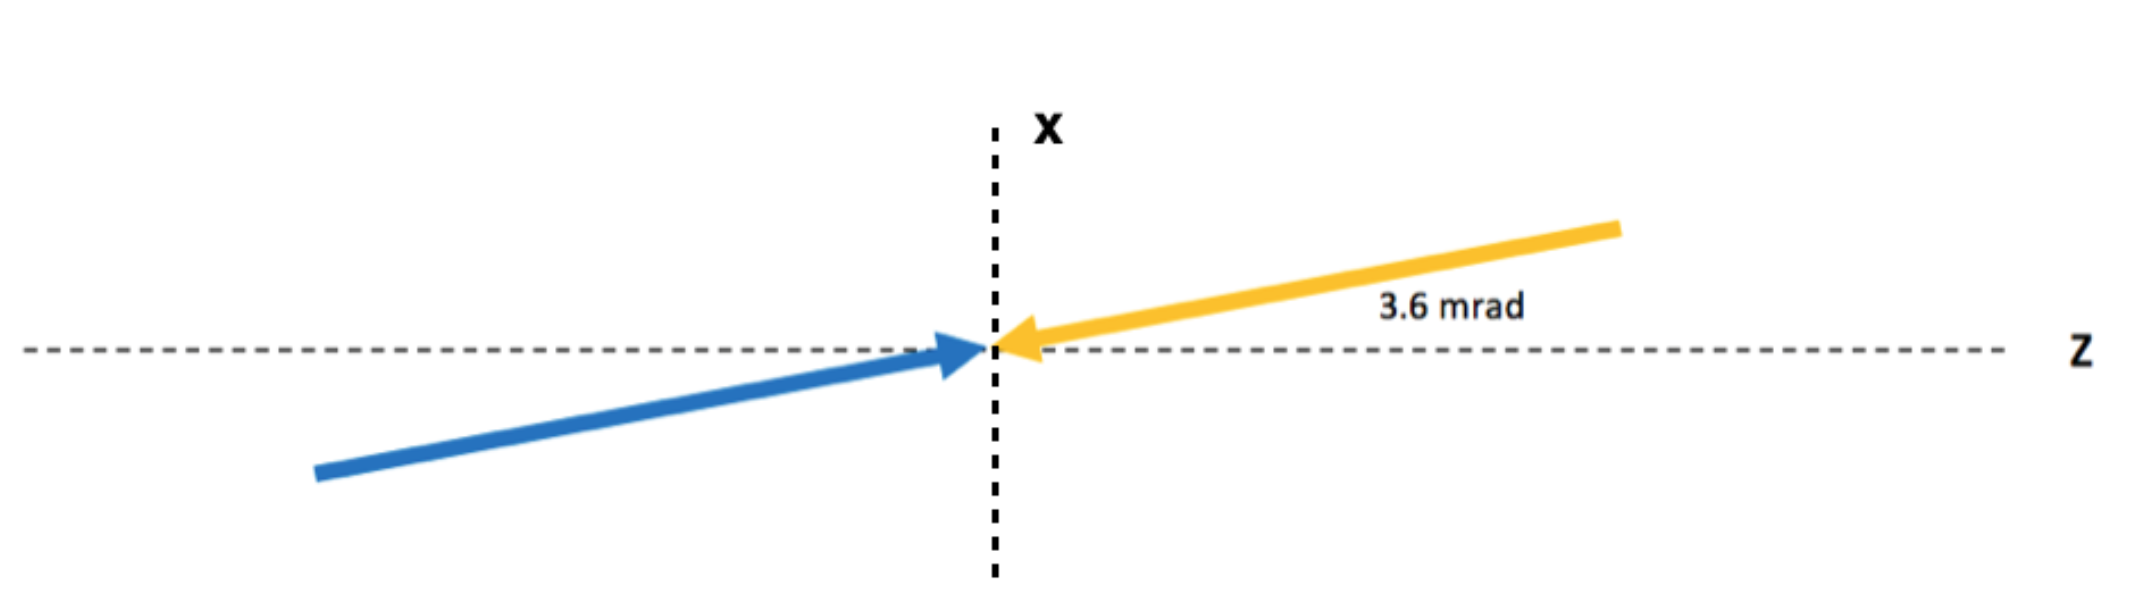
\includegraphics[width=0.75\linewidth]{figs/beam_angle.png}
\caption{Diagram illustrating the angle at which the yellow and blue beams collide relative to the longitudinal $z-$axis of the detector. The yellow beam corresponds to the Au (south-going) beam, and blue corresponds to the proton (north-going) beam. Due to a necessity of running p+Au collisions @ 200 GeV at RHIC, the beams collide at an angle of 3.6 mrad.}
\label{fig:diagram2}
\end{center}
\end{figure}

First of all, the collision vertex is significantly offset from the z-axis to which all of the PHENIX detectors are aligned. The other beam geometry effect, and the more significant of the two effects, comes from the fact that the beams are colliding at an angle of 3.6 milli-Radians in the x-z plane as show in Fig ~\ref{fig:diagram2} \cite{BNL_Run15_Operations}. The reason a non-ideal beam geometry creates an east west v2 measurement difference is because of the assumption that the ideal event plane angle is azimuthally isotropic during the event plane flattening calibration. In the translated and rotated frame where the beams are aligned with the z-axis the event plane distribution would be uniform, but in the lab frame the event plane distribution in $\phi$ would have regions of enhancement and reduction. The event plane flattening calibration algorithm restores a non-uniform distribution to a uniform one; however, if the true event plane distribution is non-uniform then forcing the measured distribution to be uniform would produce systematic errors.

We correct for the offset of the collision vertex by shifting the origin of the PHENIX global coordinate system to the true collision vertex. To correct for the effect of the beam angle, we apply a global rotation of the PHENIX coordinate to align its longitudinal axis with that of the beams. In practice, these transformations are accomplished by individually applying a global rotation and translation to every CA track, FVTX cluster, and BBCs PMT. As shown in Fig \ref{fig:fvtx_ew_rot}, applying these corrections prior to calculating $v_2$ reduces the magnitude of the east-west discrepancy but not entirely \textbf{TODO: QUANTIFY THIS.} 

Even after rotating the PHENIX global corrdinate system to be in alignment with the beam axis, due to the fact $PSi_2$ is a derived quantity, there is a residual effect from the beam rotation which still effects the $v_2$ measurement.

%To correct for the collision vertex offset effect the PHENIX detector elements must have their position calculated with respect to the collision vertex rather than the origin and to correct for the beam rotation effect the PHENIX detector elements must be rotated into the beam frame where the beam is aligned with the z-axis. As shown in Fig \ref{fig:fvtx_ew_rot}, applying these corrections to the event plane when calculating $v_2$ reduces the magnitude of the splitting but not entirely. The detector elements being in the right place in the beam frame will not completely correct the event plane bias.


\begin{figure}[!h]
\begin{center}
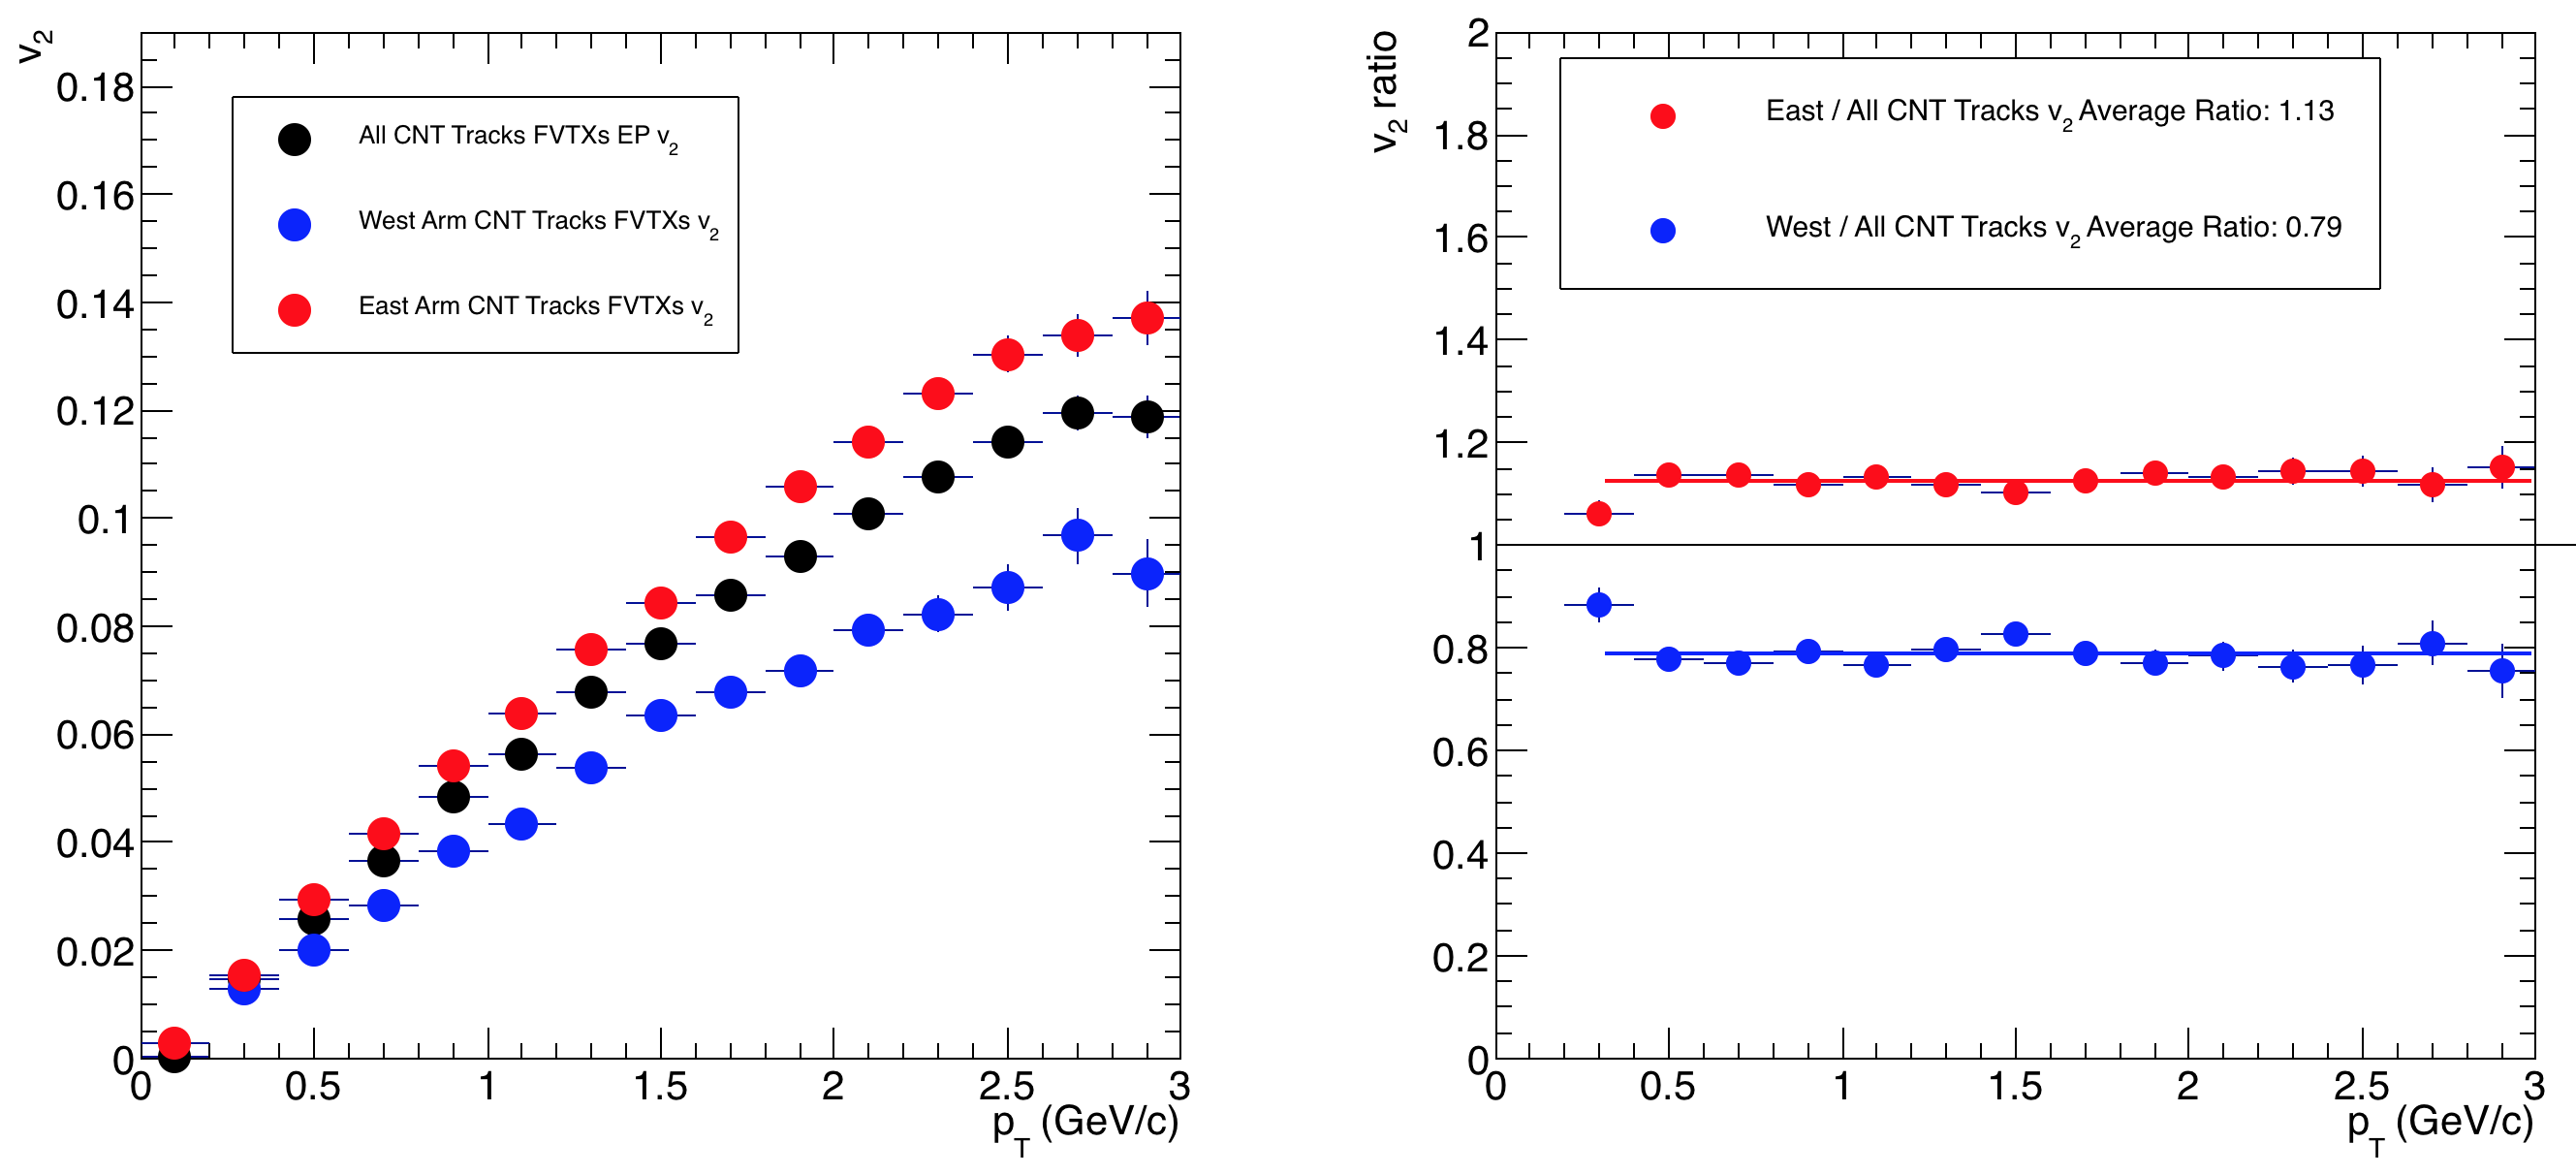
\includegraphics[width=0.85\linewidth]{figs/fvtx_vertex_rot_only.png}
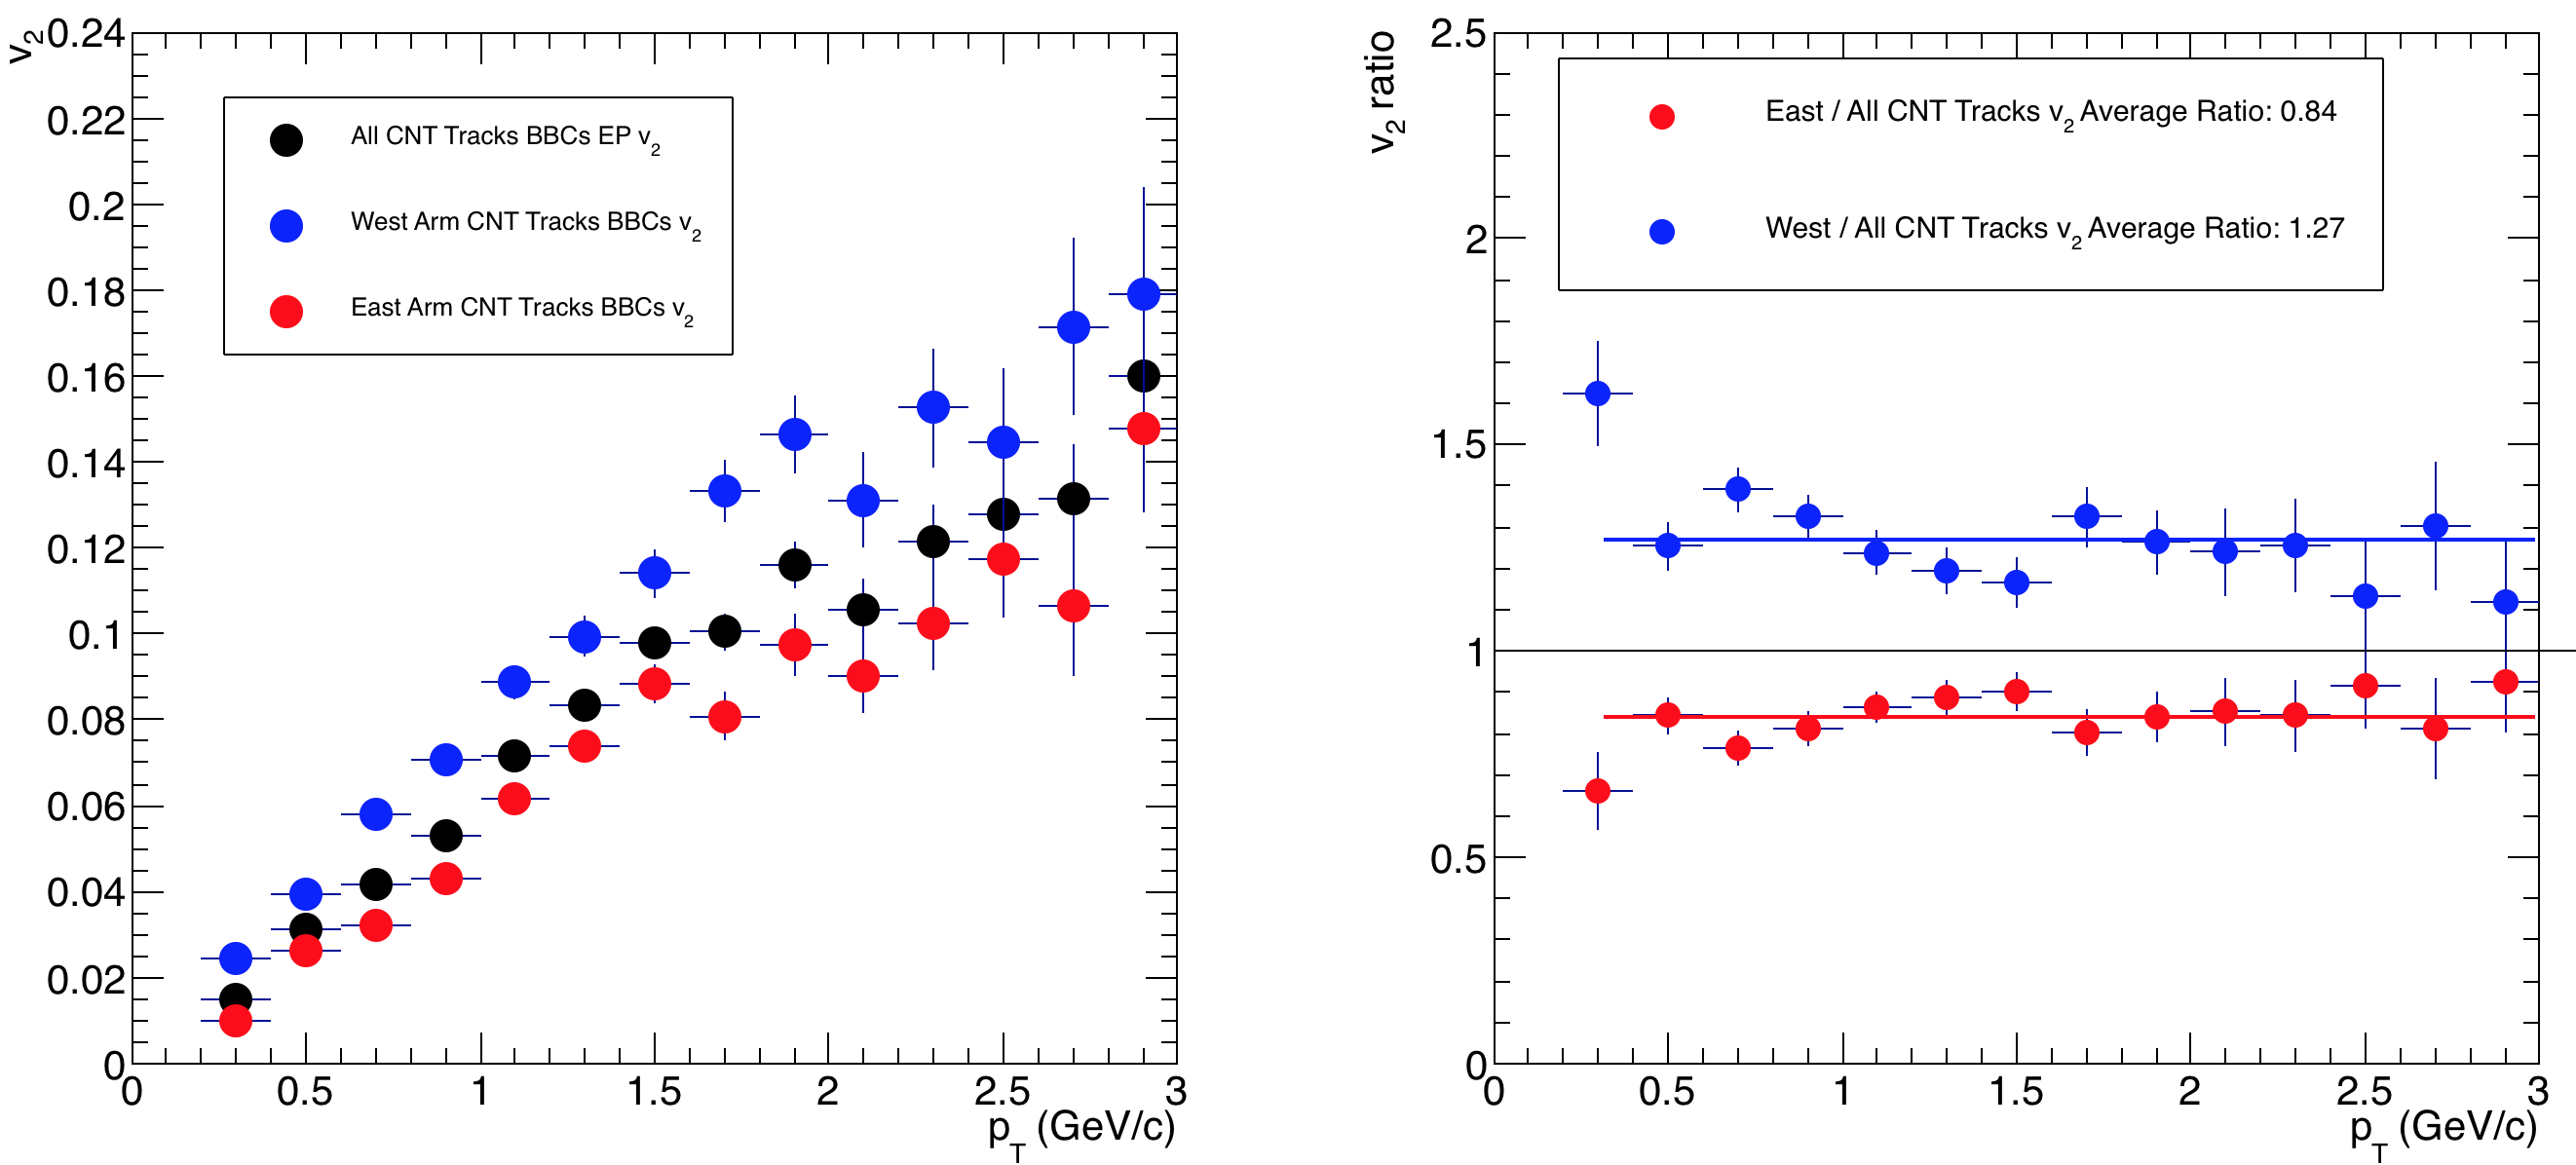
\includegraphics[width=0.85\linewidth]{figs/bbc_vertex_rot_only.png}
\caption{A corrected measurement of $v_{2}$ as a function of $p_T$ with the FVTXs (top 2 panels) and the BBCs (bottom 2 panels) event plane for the p+Au @ 200 GeV dataset. The default resolution as shown in table TBA is used. The plotting conventions are the same as described in the caption of Fig \ref{fig:fvtx_ew_default}. Even after correcting for the moving the detector elements back in the right place, it is apparent that there is still a significant splitting of the measurement although there is an improvement. For the FVTXs event plane, the east $v_2$ measurement is 13$\%$ higher on average from the all CNT track measurement and the west measurement is 21$\%$ lower on average and for the BBCs event plane, the east $v_2$ measurement is 27$\%$ higher on average and the west measurement is 16$\%$ lower on average.}
\label{fig:fvtx_ew_rot}
\end{center}
\end{figure}

To explain this effect, consider a cylindrical disk with a hole in the middle, centered about the z-axis (in analogy to the shape of the FVTX and the BBC), as shown in the left plot of Fig \ref{fig:tilt_effect}. In this geometry, all points along a ring of constant radius are at the same pseudorapidity. However, if one were to tilt that disk, the pseudorapidity of points along that ring would be $\phi$ dependent. The tilt of the disk changes its pseudorapidity acceptance and its extent. Now consider that it is not the disk that is tilted but rather the beam orientation that is tilted. The previous statements about the effect on the $\eta$ range being $\phi$ dependent still apply. 

The combination of the $\eta$ acceptance changing, and the $\eta$ distribution of charged particles not being flat means that the average amount of charged particles going through the disk would be systematically $\phi$ dependent, as illustrated in Fig \ref{fig:tilt_effect}. If the average charged particle distribution is not uniform in $\phi$, the event plane distribution will not be either. This results in the flattening procedure creating systematic effects such as the east-west $v_2$ asymmetry.

\begin{figure}
\begin{center}
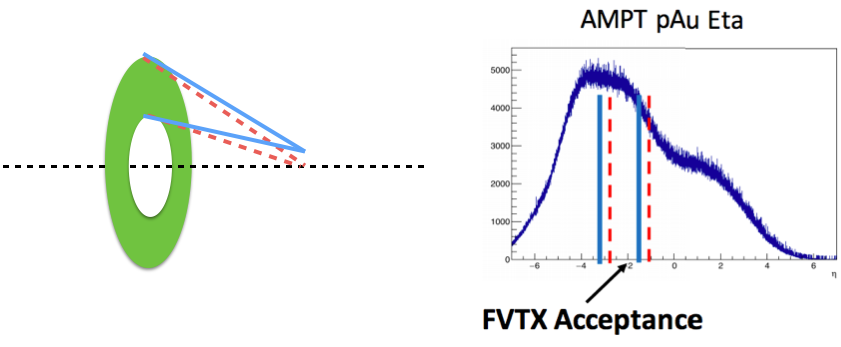
\includegraphics[width=0.95\linewidth]{figs/tilt_effect.png}
\caption{(left) Cartoon diagram illustrating $\eta$ acceptance shift due to a beam offset in one of the FVTXs layers. (right) Pseudorapidity distribution of charged particles from the AMPT Monte Carlo generator for pAu @ 200 GeV, showing the shift in $\eta$ acceptance.}
\label{fig:tilt_effect}
\end{center}
\end{figure}

In order to correct for this effect, an additional weight factor is introduced for FVTX clusters and BBC PMTs during the event plane calculation. This factor is such that hits in $\phi$ regions with systematically less particles are given a larger weight, and correspondingly, hits in $\phi$ regions with systematically more particles are weighted less. The introduction of this weighting as define below does not formally change ...
\begin{equation}
w_i = w^D_i*F(\phi,Vertex_Z)
\label{eqn:modified_weight}
\end{equation}

where $w^D_i$ is the default weighting associated with the detector element and $F(\phi,Vertex_Z)$ is the multiplicative weighting to correct for the beam geometry. $F(\phi,Vertex_Z)$ is dependent on $Vertex_Z$ in addition to $\phi$ because $\eta$ is dependent on the collision vertex. One can analytically calculate this $\phi$ dependent weight factor using the geometry of the FVTXs and BBCs as well as using the $\eta$ distribution of charged particles. Unfortunately, the $\eta$ distribution of charged particles in pAu @ 200 GeV has not been measured by an experiment so we must rely on models which may be inaccurate.

\begin{figure}[h!]
\begin{center}
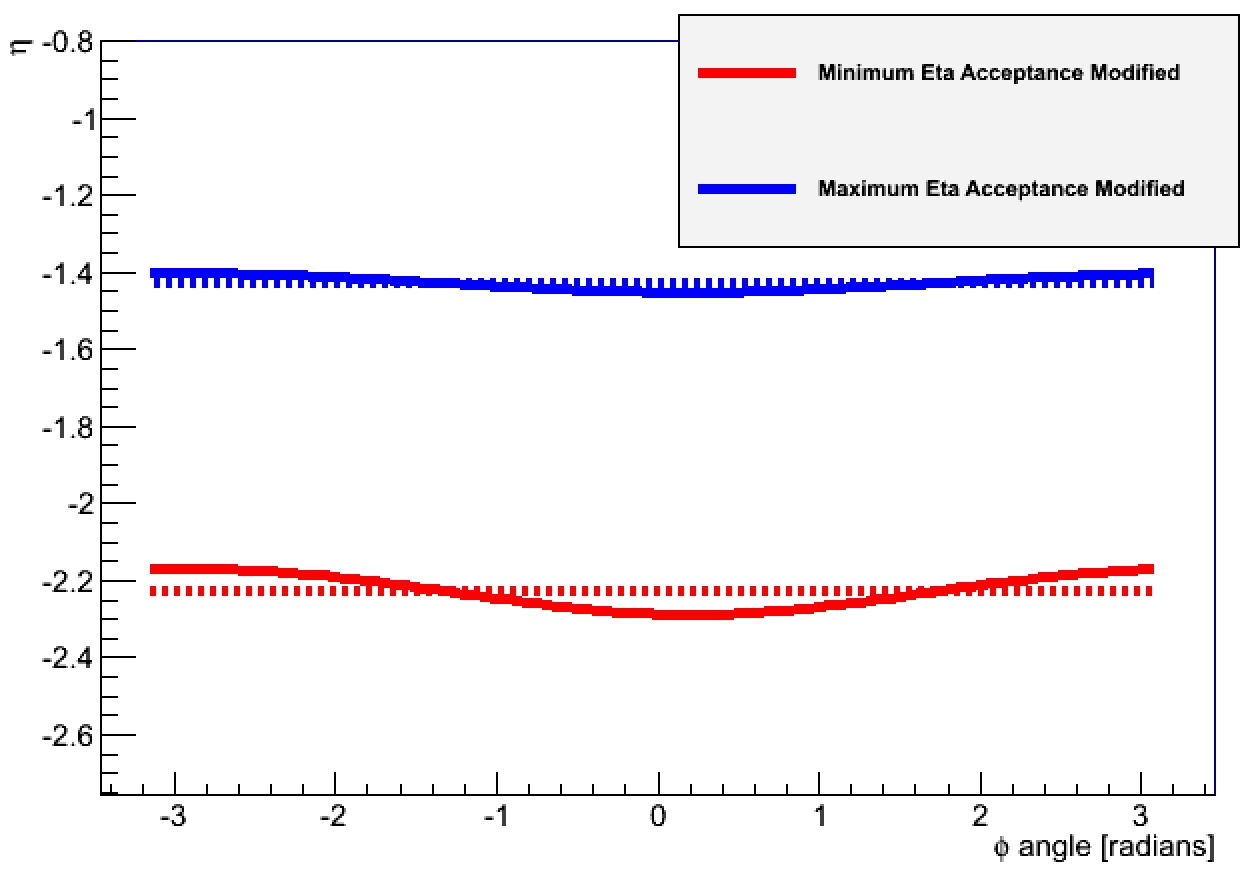
\includegraphics[width=0.47\linewidth]{figs/eta_modification.png}
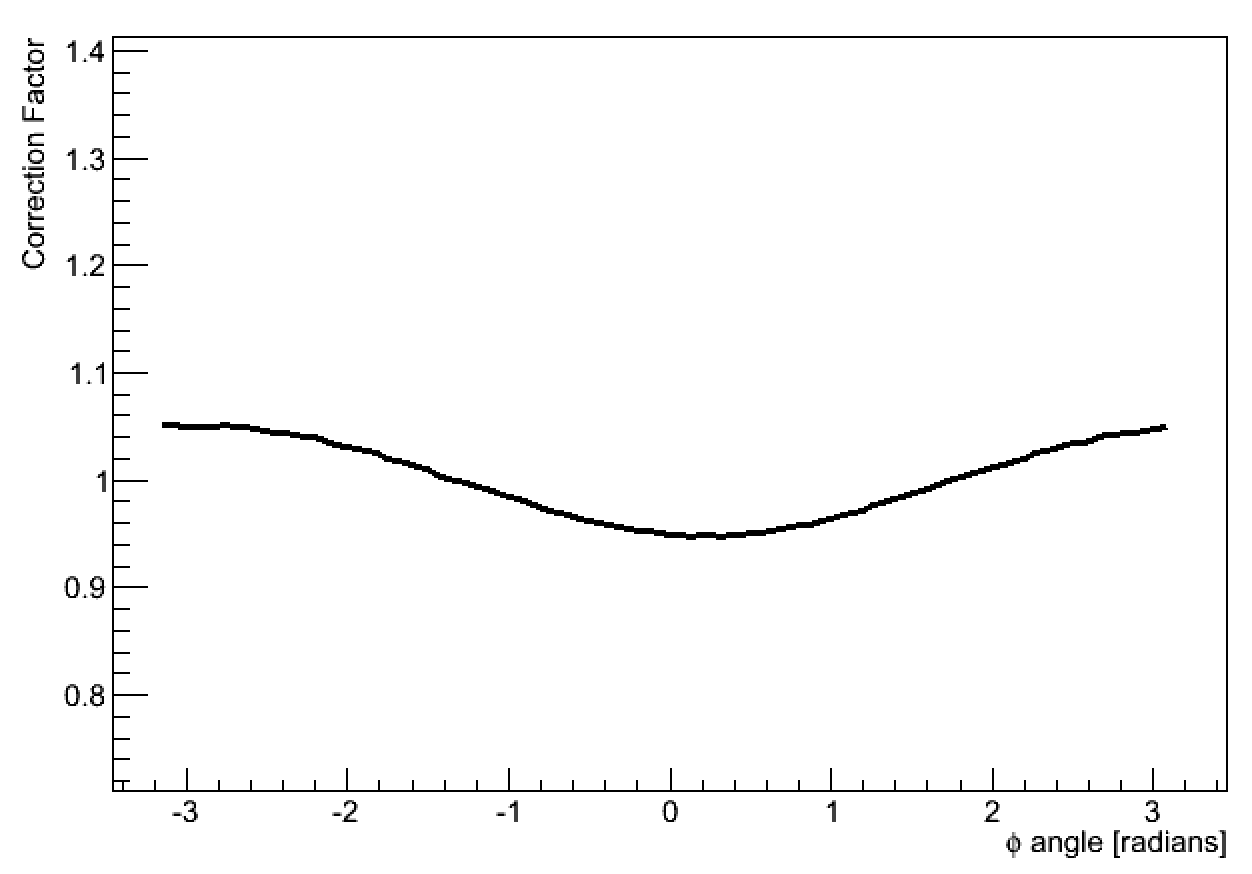
\includegraphics[width=0.47\linewidth]{figs/analytic_correction.png}
\caption{The left is the modification of the $\eta$ acceptance as a function of $\phi$ for the FVTX first layer. The right is the calculated correction factor from this.}
\label{fig:analytic_corr}
\end{center}
\end{figure}

Another way to determine the weight factor is to use a data driven method of measuring to what extent each $\phi$ region in a detector is has systematically more or less particles. Then an inverse weighting based on this measurement is applied to the $\phi$ regions to correct the detector's $\phi$ distribution to uniformity. The precise implementation of measuring and applying the uniformity of the $\phi$ regions in a detector will be examined further in the following sections.

\subsection{FVTX Inverse Phi Weighting}
\label{sec:FVTX_inv_phi_weight}
For this method, the weight factor is determined by plotting all hits in a cylindrical disk detector vs $\phi$, normalizing this distribution to one, and then inverting it. When applying this weight factor to the data, it will produce uniform hit distributions in $\phi$ in the detectors it is applied to. This will, in turn, make the event plane distribution more uniform when measured in those detectors, thus correcting for the effect. The added benefit of using this method is also correcting for hot and cold $\phi$ regions in the detector. In order to get rid of significant hot or cold $\phi$ regions, $\phi$ regions with weight factors greater than 1.5 or less than 0.5 are set to 0.0. This correction is done for each FVTX layer, in z-vertex bins, and per run. The multiplicative weight function $F(\phi,Vertex_Z)$ for the FVTX disks is defined as 
\begin{equation}
F(\phi,Vertex_Z,layer) = \frac{\left<N_{CLUS}(Vertex_Z,layer)\right>}{N_{CLUS}(\phi,Vertex_Z,layer)},
\end{equation}
where $N_{CLUS}(\phi,Vertex_Z,layer)$ is the number of FVTX clusters as a function of $\phi$, $Vertex_Z$, and FVTX layer and $\left<N_{CLUS}(Vertex_Z,layer)\right>$ is the $\phi$ average of the number of clusters. The weighting can be seen in Fig \ref{fig:fvtx_weighting}. A comparison between the FVTX weighting and the analytic correction is shown. The good agreement indicates the validity of the weighting.

\begin{figure}[h!]
\begin{center}
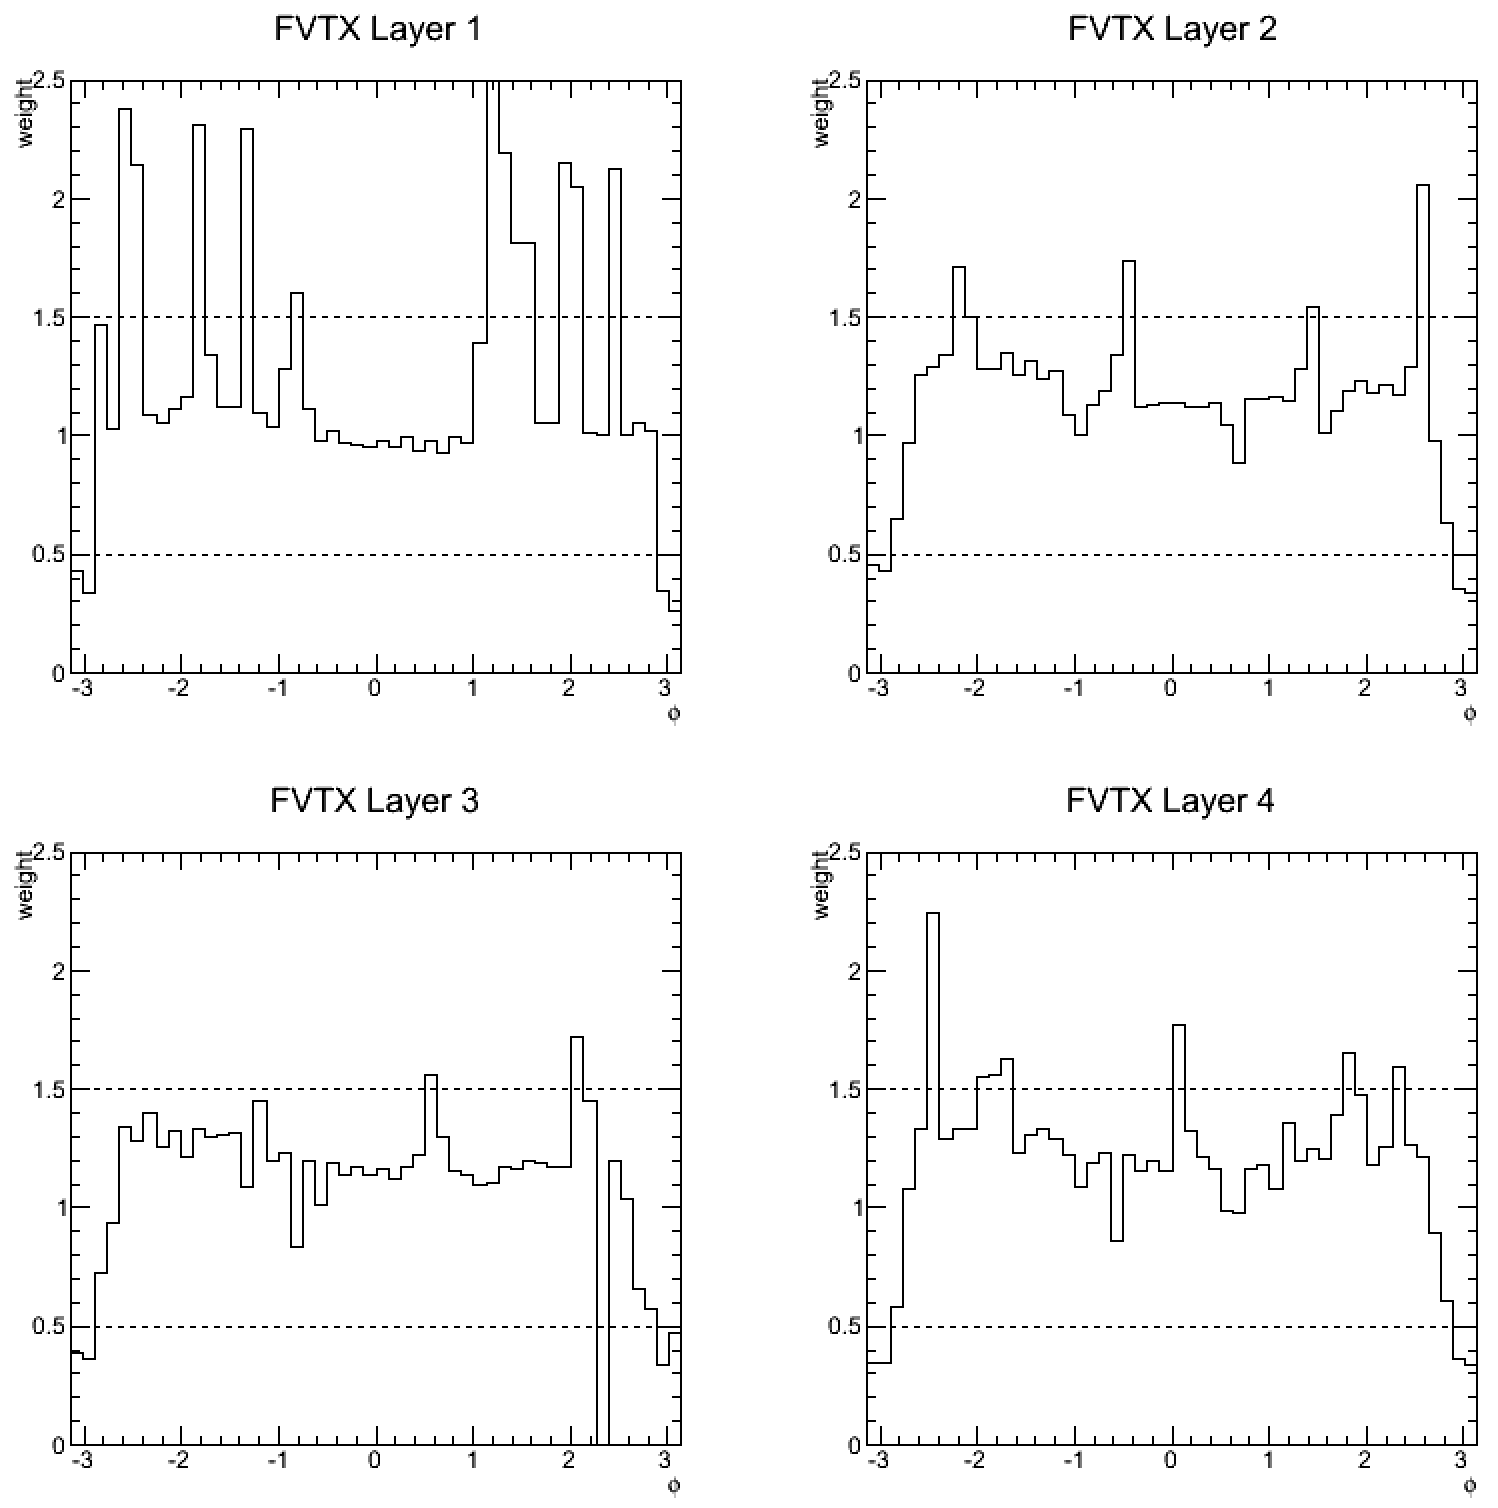
\includegraphics[width=0.75\linewidth]{figs/fvtx_weighting.png}
\caption{These 4 panels show the FVTX $\phi$ dependent cluster weighting when calculating the FVTX event plane for each layer separately for events with a collision vertex in z is around 0. As you can see there are some $\phi$ regions where weight factor is outside of the dotted line bounds. This indicates that either there was a severe deficit of clusters measure in the region or excess. Later, we will examine the effect of keeping these regions or cutting them out on the $v_2$ measurement.}
\label{fig:fvtx_weighting}
\end{center}
\end{figure}
\begin{figure}[!h]
\begin{center}
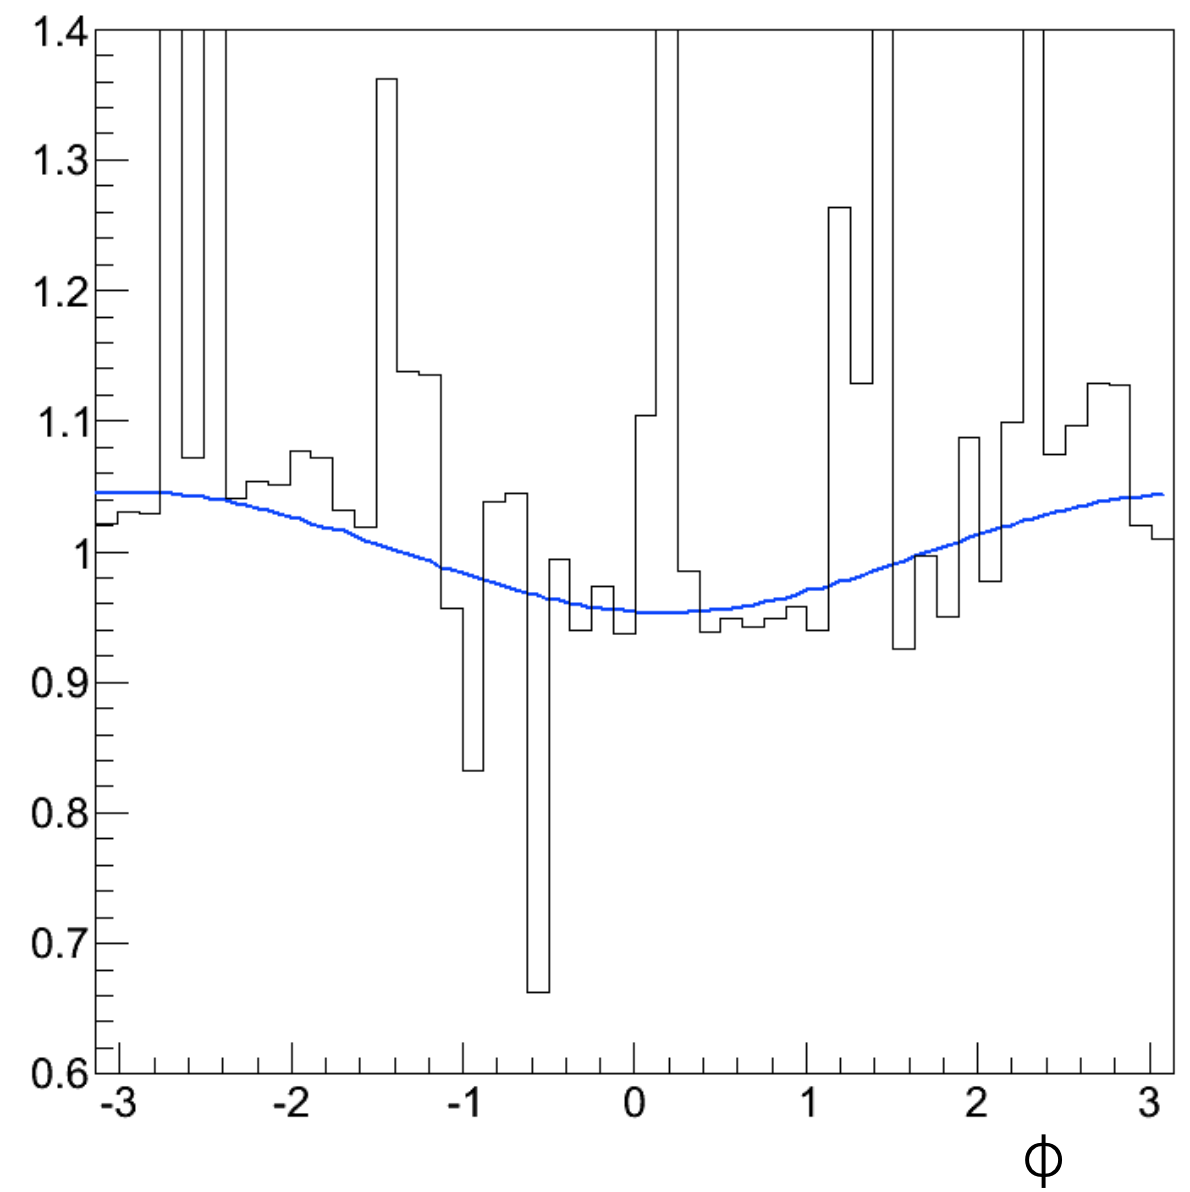
\includegraphics[width=0.5\linewidth]{figs/comparison_of_weights.png}
\caption{The black is the FVTX weighting and the blue is the analytic weighting. They have good agreement.}
\end{center}
\end{figure}

\subsection{BBC Charge Weighting}
\label{sec:bbc_charge_weight}
For the BBC, another data driven method is used to correct for the non-uniform particle distribution. Using the distribution of particles in the BBC from the Run15 pp dataset as a baseline, one can apply an inverse weighting much like the one described in the previous paragraph. In the pp dataset, there was no issue with beam colliding at an angle and the average charge across all 64 PMTs in the BBCs is uniform. In this method, the multiplicative weight function $F(PMT,Vertex_Z)$ for the BBCs is defined as:
\begin{equation}
F(PMT,Vertex_Z) = \frac{\left<N^{pp}_{Charge}(Vertex_Z)\right>}{\left<N^{pAu}_{Charge}(PMT,Vertex_Z)\right>},
\end{equation}
where $<N^{pp,pAu}_{Charge}(PMT,Vertex_Z)>$ is the event averaged charge as a function of PMT and $Vertex_z$ for the pp and pAu datasets respectively. 
This weight function is shown in Fig \ref{fig:bbc_weight_function} and is applied directly to the event plane calculation using Eqns \ref{eqn:modified_weight} and \ref{eqn:bbc_ep_eqns}. 
Although the weight function could be defined as a function of $\phi$ like in the FVTX case, the positions of the PMTs in the BBC are fixed and it is more direct to take the ratio between PMTs.

\begin{figure}[h!]
\begin{center}
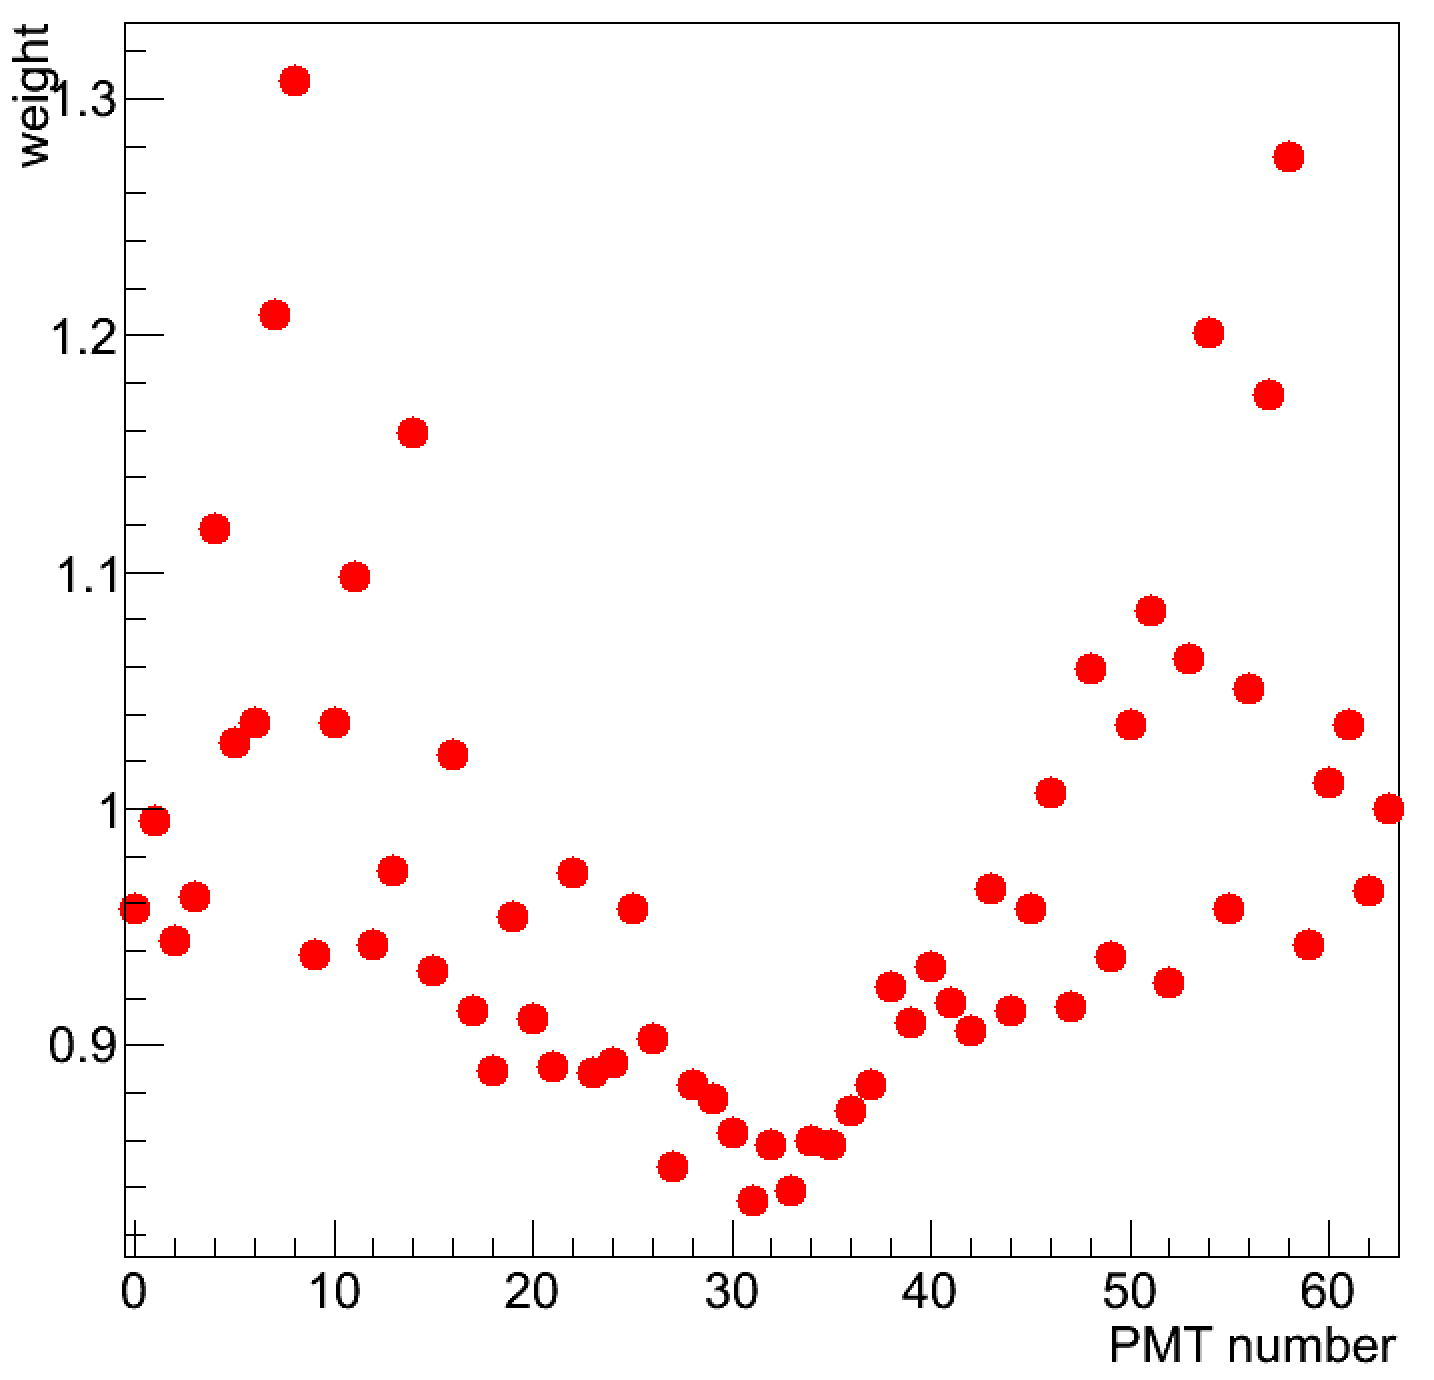
\includegraphics[width=0.5\linewidth]{figs/pmt_ratio_weight.png}
\caption{Shown here is BBC the multiplicative weight factor $F$ used when calculating the modified event plane for events where the collision vertex in z is around 0. The y-axis is the weight factor and the x-axis is the PMT number for the BBCs (there are 64 total in the BBCs). }
\label{fig:bbc_weight_function}
\end{center}
\end{figure}

One effect of using this weighting method is that it will make the distribution of particles in the BBC in $\phi$ and $\eta $ uniform. This can be illustrated by looking at Fig \ref{fig:bbc_pmt_phi_pp_pau}. It is apparent that the p+p average charge is much more uniform than the p+Au average charge as a function of $\phi$ and ring. After applying the p+p/p+Au ratio weighting, which is essentially dividing the left plot by the right plot in Fig \ref{fig:bbc_pmt_phi_pp_pau}, the PMT charges in ring 1 for the p+Au dataset will be deweighted such that their corrected average charge will be uniform in $\phi$ and in agreement with the average charge for the other rings. If all the BBC rings have the same average charge, this means that the average charge as a function of $\eta$ for the BBC will be approximately uniform. This is a reason why for the BBC this method (p+p/p+Au ratio weighting) is preferred, because the variations in the average charge between the rings are normalized. One could apply the FVTX method of inverse $\phi$ weighting by inverting the right plot of Fig \ref{fig:bbc_pmt_phi_pp_pau} to find the weight function. However, although using only the p+Au dataset would normalize the average charge as a function of $\phi$ it would not normalize the charge as a function of $\eta$. Both methods applied to the data are shown in the next section but the p+p/p+Au ratio method does better.

\begin{figure}[h!]
\begin{center}
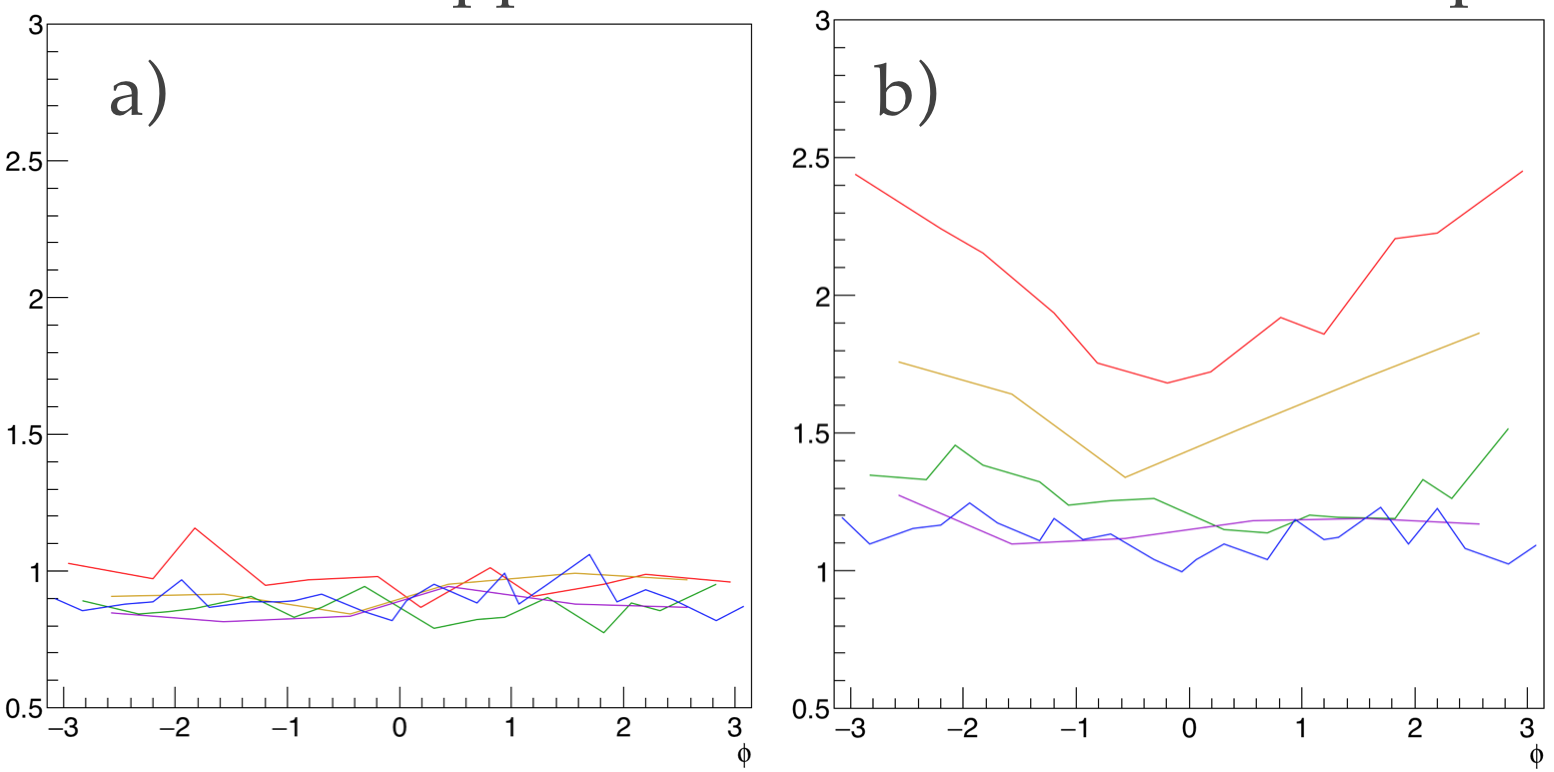
\includegraphics[width=0.75\linewidth]{figs/pp_pau_bbc_comparison.png}
\caption{These plots depict the average PMT charge per event versus $\phi$ in the a) the p+p @ 200 GeV and b) p+Au @ 200 GeV. The PMTs are separated by color which corresponds to rings of approximate common radius as shown in Fig \ref{fig:bbc_rings}. The left plot shows near uniformity as a function of $\phi$ and ring. However, the right plot shows a significant deviation from uniformity especially for the innermost rings (rings 1 and 2) there is. In addition to the $\phi$ variation for the right plot, the innermost rings have the largest average charge when compared to the other rings. This is in part due to the fact the inner most rings cover the a slightly larger $\eta$ range. However, the innermost rings in the left plot also cover the largest $\eta$ range and do not exhibit this separation in rings. }
\label{fig:bbc_pmt_phi_pp_pau}
\end{center}
\end{figure}

\subsection{Applying Weighting to v2}
When applying the sophisticated weighting to the $v_2$ measurement, we can quantify how much the weighting corrects the east west $v_2$ asymmetry. This quantity is calculated by: 
\begin{equation}
ratio v_2 = \frac{\sum_{p_T}{eastv_2(p_T)}}{\sum_{p_T}{westv_2(p_T)}},
\end{equation}
and should be closest to 1.0 if the weighting is working.
Shown in Fig \ref{fig:fvtx_corr_summary} is the correction summary for the FVTX $v_2$ measurement. The 20\% east west deviation is shown in the first column as the black circle. The red, blue and green analytic, inverse $\phi$ weighting, and inverse $\phi$ weighting respectively all bring the ratio quantity much closer to 1.0 indicating the weighting techniques are working. This last statement is true given that we exclude the third layer of the FVTX from our calculation. The rationale for this exclusion is due to FVTX layer three's unusual behavior in relation to the other FVTX layers. As we go from layer 1 to layer 4 the east west ratio quantity generally is trending down except for layer 3. Most likely there is something wrong with the layer data due to electronic or detector problems. 
\begin{figure}[!h]
\begin{center}
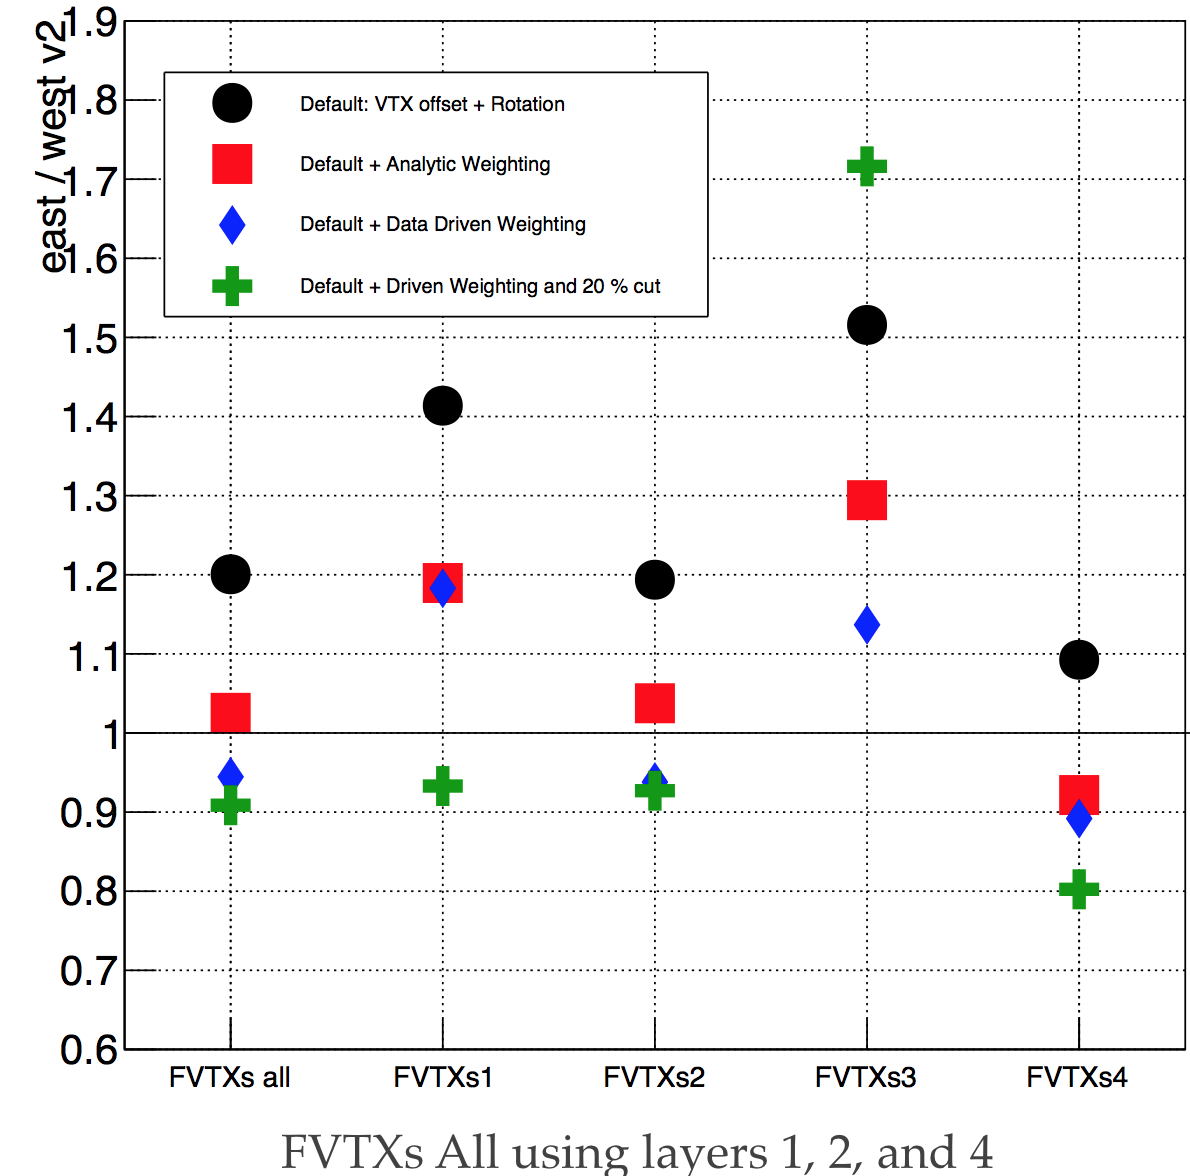
\includegraphics[width=0.5\linewidth]{figs/fvtx_correction_summary.png}
\caption{Plotted is the FVTX correction summary where the y-axis is the east/west $v_2$ ratio and the x-axis is the different subset of clusters used to calculate the $v_2$. The black markers are with the default corrections as shown in Fig \ref{fig:fvtx_ew_default}. The red boxes are the corrections with the analytic weighting shown in Fig \ref{fig:analytic_corr}. The blue diamonds are the FVTX inverse $\phi$ weighting as shown is section \ref{sec:FVTX_inv_phi_weight}. Finally, the green crosses are the same as the blue diamonds except a hot cold filter of 20\% was applied additionally. The first column is using all the FVTX layers except for the 3rd layer (which will be explained more later). So the first columns should be approximately the average of columns 2, 3, and 5. Columns 2 through 5 show the ratio calculated from clusters only in that layer. The east west ratio is the worst in layer 3 across all correction methods which is why it was excluded from the first column. The blue, red and green corrections all give equivalent levels of correction.}
\label{fig:fvtx_corr_summary}
\end{center}
\end{figure}

\begin{figure}[!h]
\begin{center}
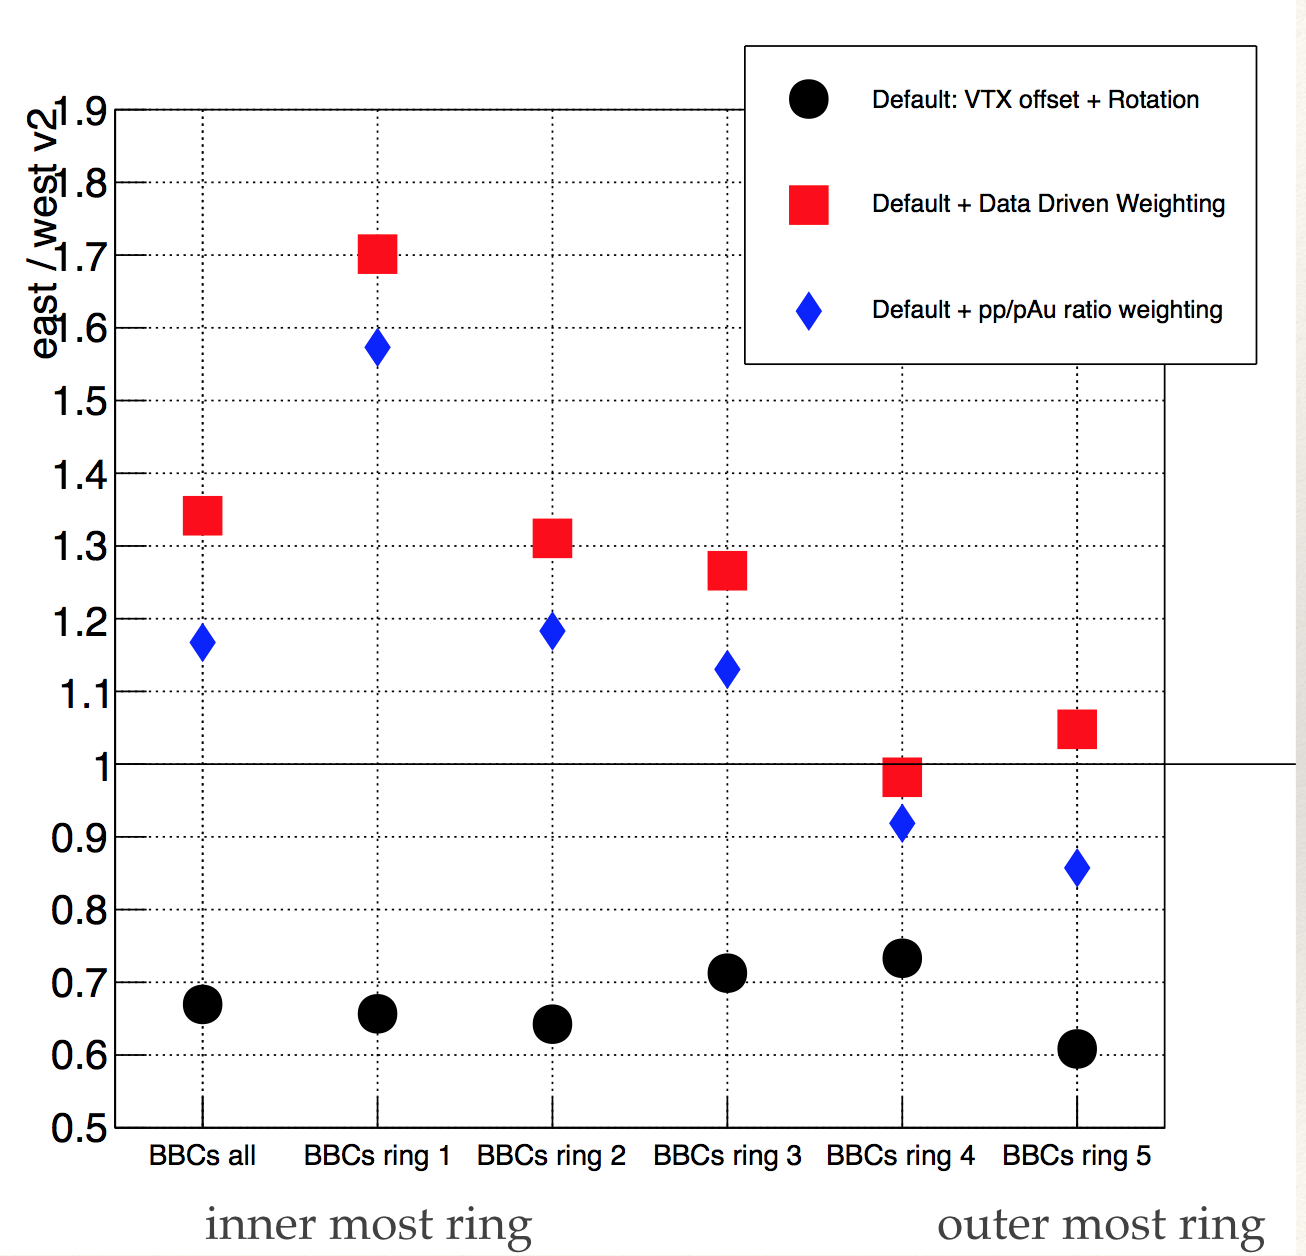
\includegraphics[width=0.5\linewidth]{figs/bbc_correction_summary.png}
\caption{Plotted is the BBC correction summary where the y-axis is the east/west $v_2$ ratio and the x-axis is the different subset of PMTs used to calculate the $v_2$. The black markers are with the default corrections as shown in Fig \ref{fig:fvtx_ew_default}. The red boxes are the corrections with the analytic weighting shown in Fig \ref{fig:analytic_corr}. Finally, the blue diamonds are the BBC inverse $\phi$ charge weighting as shown is section \ref{sec:bbc_charge_weight}. The first column is the quantity calculated from all PMTs. columns 2 through 6 are using PMTs from certain rings as defined in Fig \ref{fig:bbc_rings}. Ring one is the hardest to correct. The first column should approximately be the average of all the other columns.}
\label{fig:bbc_corr_summary}
\end{center}
\end{figure}

Fig \ref{fig:fvtx_corrected_best} shows the $v_2$ vs $p_T$ with the green cross correction from Fig \ref{fig:fvtx_corr_summary}. This figure also shows $v_2$ vs $p_T$ with the blue diamonds from Fig \ref{fig:bbc_corr_summary}. Although the east west ratio does not become exactly 1.0, a ratio value of $\pm$10 $\%$ of 1.0 is good enough to reduce our systematics errors. This is true for the FVTX points but for the BBC points we never found a weighting scheme to correct the east west ratio to be between 0.9 and 1.1. This is in part why the primary measurement is done using the FVTX.

\begin{figure}[!h]
\begin{center}
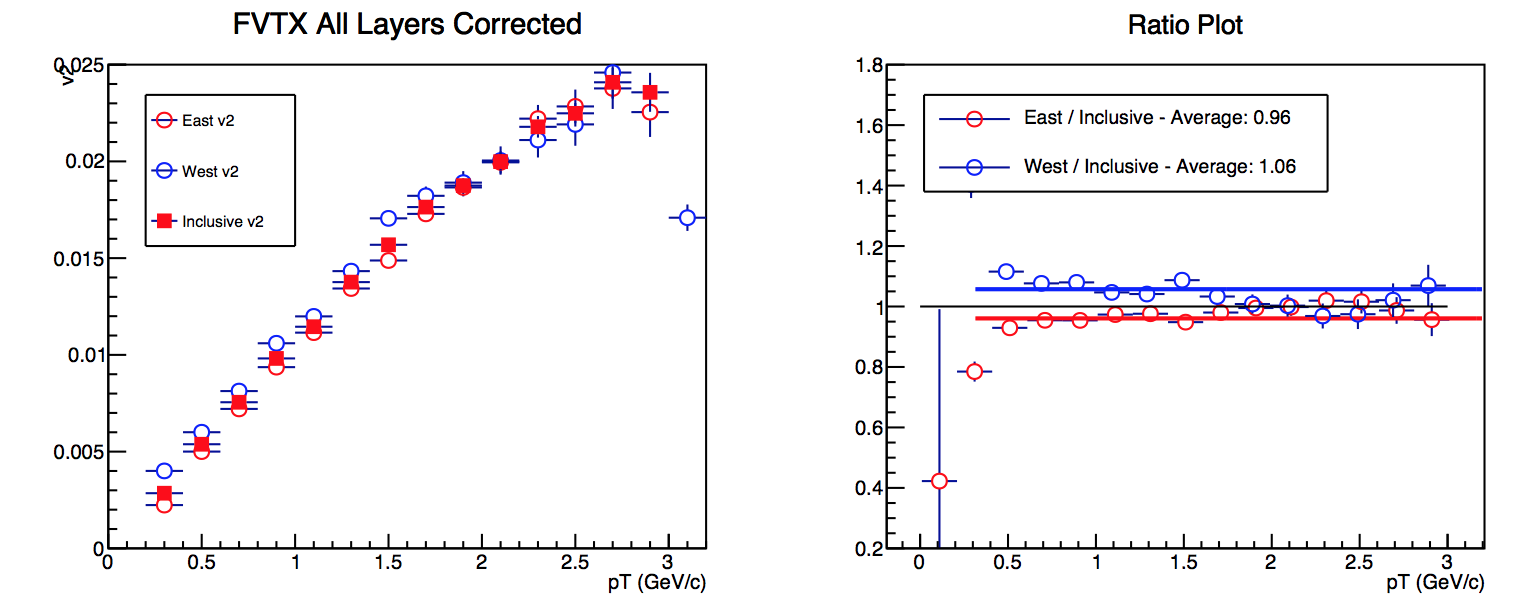
\includegraphics[width=0.75\linewidth]{figs/fvtx_corrected.png}
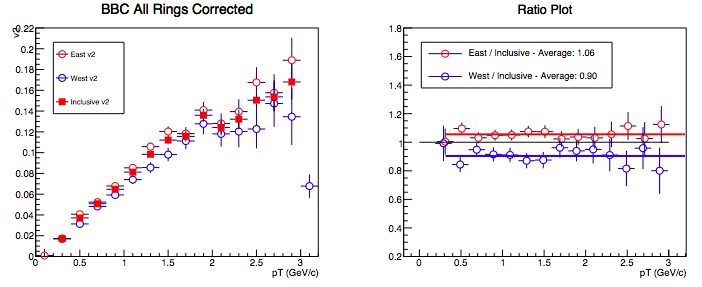
\includegraphics[width=0.75\linewidth]{figs/bbc_pp_correction.png}
\caption{The top plots are FVTX event plane measurement corrected with inverse $\phi$ weighting and 20 $\%$ cut. FVTX layer three is excluded. This correction effectively eliminates the east west difference shown on the right.. The bottom plots are BBC event plane measurement corrected with inverse $\phi$ weighting and 20 $\%$ cut. This correction reduces the east west difference significantly.}
\label{fig:fvtx_corrected_best}
\end{center}
\end{figure}
\clearpage
%\begin{figure}[!h]
%\begin{center}
%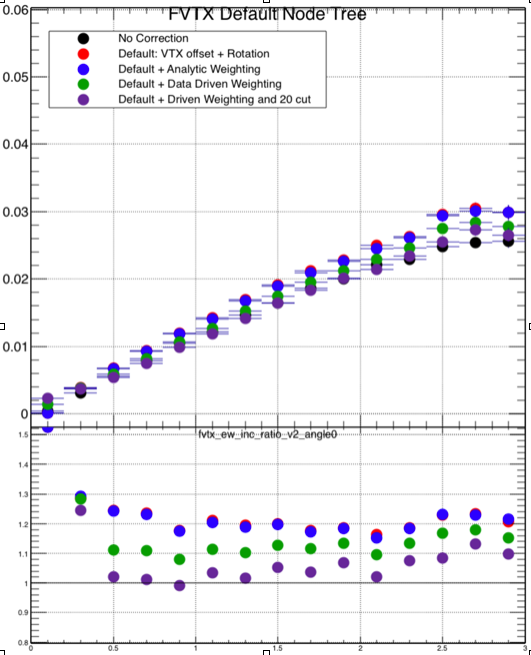
\includegraphics[width=0.5\linewidth]{figs/fvtx_incl_v2_comparison_corrections.png}
%\caption{}
%\end{center}
%\end{figure}

\section{Systematic Uncertainties}
The main sources of systematic uncertainty in the $v_2(p_T)$ measurement are: (1) track background from photon conversion and weak decays, whose magnitude we determine at 2\% relative to the measured $v_2$ by varying the spatial matching windows in the PC3 from 3$\sigma$ to 2$\sigma$; (2) Multiple collisions per bunch crossing (i.e., event pile-up) that are observed to occur at an average rate of 8\% in the 0\%-5\% central p+Au collisions. Low luminosity and high-luminosity subsets of the data were analyzed separately and the systematic uncertainty in the $v_2(p_T)$ value is determined to be asymmetric  $^{+4\%}_{-0\%}$, since the $v_2$  values were found to decrease in the events that contain a larger fraction of pile-up, an example of a pile up event is shown in Fig \ref{fig:pile_up_example}; (3) Non-flow correlations from elementary processes that enhance the $v_2$ values, whose contribution we estimate from Fig.~\ref{fig:non_flow}, assigning a $p_T$-dependent asymmetric uncertainty with a maximum value of $^{+0}_{-23}\%$ for the highest $p_T$ bin. This can be compared to the corresponding $^{+0}_{-9}\%$~\cite{Adare:2014keg} and $^{+0}_{-7}\%$~\cite{PhysRevLett.115.142301} systematic uncertainties in d+Au and $\mbox{$^3\text{He}$+Au}$ collisions, respectively; (4) The asymmetry between the east ($\pi/2 < \phi < 3\pi/2$) and west ($-\pi/2 < \phi < \pi/2$) acceptance of the detectors due to an offset of 3.6 mrad between the colliding beams and the longitudinal axis of PHENIX, necessary for running p+Au at the same momentum per nucleon. We applied a corresponding counter-rotation to every central arm track and detector element in the FVTX and BBC, which were also reweighted to restore their uniformity in azimuth. We assign a value of $5\%$ for this systematic uncertainty by taking the difference of $v_2$ as measured independently in the east and the west arms after applying the above corrections; (5) The difference in the $v_2(p_T)$ values when measured independently using the BBC-S and FVTX event planes, which differ by $\pm$3\%. 

Table~\ref{t:sys} summarizes of all these systematic
uncertainties, categorized by type:

(A) point-to-point uncorrelated between $p_T$ bins,

(B) point-to-point correlated between $p_T$ bins,

(C) overall normalization uncertainty in which all points are scaled by the same multiplicative factor.

\begin{table}[!h]
  \begin{center}
  \caption{\label{t:sys}Systematic uncertainties given as a percent of the $v_2$ measurement. Note that the non-flow contribution is $p_T$ dependent and the value here quoted corresponds to the highest measured $p_T$.}
    \begin{tabular}{ccc}
      \hline
      \hline
      Source& Systematic Uncertainty & Type \\ \hline
      Track Background &2.0\%& A\\ 
      Event Pile-up    &$^{+4}_{-0}\%$& B\\
      Non-Flow    &$^{+0}_{-23}\%$& B\\
      Beam Angle &5.0\%& C\\  
      Event-Plane Detectors & 3\% & C\\
    \hline
    \hline
    \end{tabular}
   \end{center}
 \end{table}

\subsection{Pile Up}
Pile up events are where two or more collisions occur with in the same bunch crossing which skew the elliptic flow measurement. Pile up events are an issue for this analysis because they:

(1) are erroneously included into the 0-5\% centrality selection due to two smaller collisions looking like a larger collision,

(2) and reduce the value of $v_2$ because one collision's event plane angle will have nothing to do with the other collisions event plane and will reduce the signal.

In order to filter pile up events we can look at the distribution of BBC PMT timing values as seen in Fig \ref{fig:pile_up_example}. We can come up with an algorithm to efficiently filter pile up events by analyzing the BBC PMT timing value distribution event by event. When the $v_2$ values are compared with and without the filter, a difference of 4\% is seen.

\begin{figure}[!h]
\begin{center}
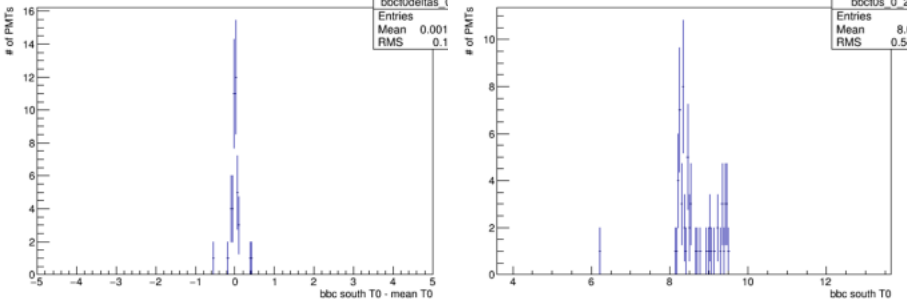
\includegraphics[width=0.8\linewidth]{figs/example_pile_up_event.png}
\caption{The distribution of BBC PMT timing values. The x-axis is the difference between the southern BBC PMT t0 - the mean t0 in the south. The left plot is an example of a normal event, the right plot is an example pile up event. A normal event is strongly peaked at 0. A pile up event has a broad distribution and may not be centered at 0. Pile up events are when 2 or more collisions happen in the same crossing.}
\label{fig:pile_up_example}
\end{center}
\end{figure}

\subsection{Event-Plane Detectors}
When measuring the $v_2$ with two different event plane detectors, the difference in the measured $v_2$ is taken to be a systematic uncertainty. 
\subsection{Track Background}
The set of tracks that are used in this analysis come from central arm tracks which are known to have a track background of 2.0\%.
\subsection{Non-Flow}
A short introduction on non-flow, may be placed in a different location later.
Non-flow is the catch all term used to categorize all types of long range angular correlations which are not the signal of hydrodynamic flow that this is analysis is seeking to measure. In effect, non-flow is the background noise to the signal of hydrodynamic flow. There are several know sources of non-flow:

(1) hard scattering events producing dijets,

(2) initial state correlations between target and projectile,

(3) decay chains of exotic particles.

(4) momentum conservation.

The contribution to the correlation function from non-flow source (1) can be seen in Fig \ref{fig:jet_corr_example}. The near-side peak at (0,0) is from the cone of particles in a single jet all having small differences in $\eta$ and $\phi$. The away-side ridge at $\phi$ = $\pi$ is from taking the differences between to the two distinct jets. The two jets are geometrically located 180 degrees apart in $\Delta\phi$ but have a smeared distribution $\Delta\eta$. This correlation function distribution produces a substantial $c_2$ very similar to the hydrodynamic flow signal we are seeking. In order to minimize the contribution of dijet events, standard flow analysis procedure is to limit the data analysis to regions outside of the red dotted lines seen in Fig \ref{fig:jet_corr_example} ($|\Delta\eta| > \eta_{min}$, where $\eta_{min}$ is usually of order 1.0 units of psuedorapidity).

\begin{figure}
\begin{center}
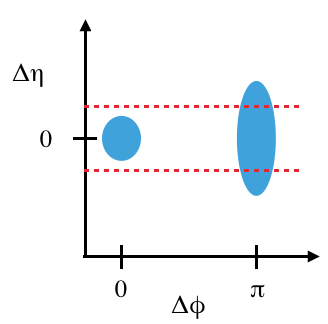
\includegraphics[width=0.5\linewidth]{figs/jet_corr_example.png}
\caption{Plotted here is the 2D profile of a correlation function in $\Delta\eta \Delta\phi$ space of a dijet event. The red dotted lines represent the exclusion zone in $\Delta\eta$ where to  make the measurement to reduce non-flow contributions.}
\label{fig:jet_corr_example}
\end{center}
\end{figure}

In order to estimate the degree of presence of non-flow, we can measure the $c_2$ from p+p events which should be devoid of any hydrodynamic flow but should have many of the sources of non-flow present. In order to compare p+p with p+Au we must scale up the p+p quantity by the dilution factor defined in eq \ref{eq:dilute}.
The scaled down reference $c_{2}$ is shown as blue squares in Fig.~\ref{fig:non_flow}, panel (a). The ratio of $c_2$ in the scaled-down p+p reference to that in p+Au is shown in panel (b). From this ratio, as calculated in \ref{eq:dilute}, it can be seen that the relative correlation strength in p+Au from elementary processes is at most 23$\%$ at the highest $p_T$. Since this procedure constitutes an approximation to quantify the non-flow correlation strength, it is not subtracted from the total signal, instead it is treated as a source of systematic uncertainty. Even though the p+Au and the p+p baseline data were collected in different years, where potential changes in detector performance could affect our results, it was verified that using p+p data from various run periods has an effect of at most 3$\%$ on the calculated non-flow contribution.
\begin{equation}
c_{2}^{{\rm pAu \; elementary}}(p_{T}) \simeq c_{2}^{p+p}(p_{T})
\frac{\left( \sum Q^{{\rm \text{BBC-S}}} \right)_{p+p}}
{\left( \sum Q^{{\rm \text{BBC-S}}} \right)_{{\rm pAu}}
}.
\label{eq:dilute}
\end{equation}

\begin{figure}[!h]
\begin{center}
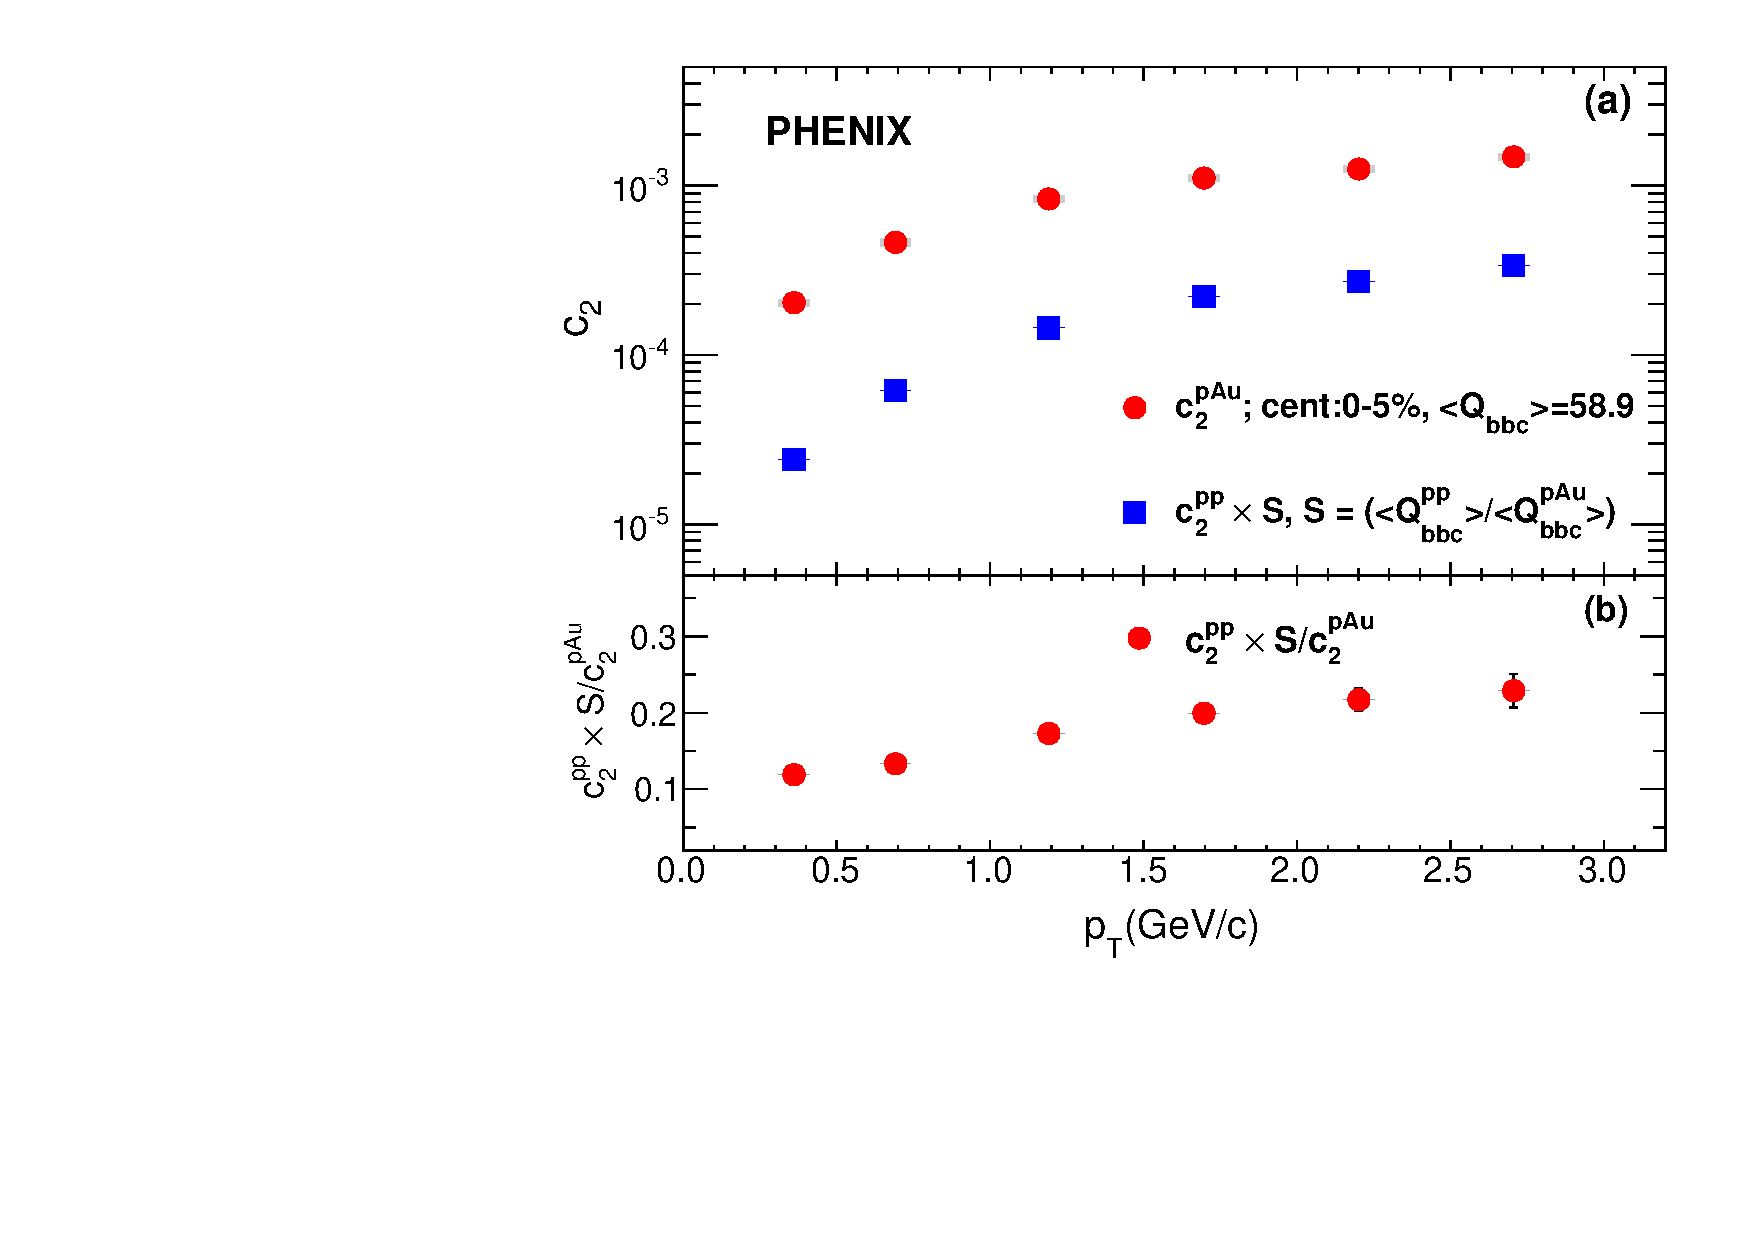
\includegraphics[width=0.6\linewidth]{figs/non_flow.pdf}
\caption{(a) The second order harmonic coefficients $c_2(p_T)$ for long range angular correlations in
0\%--5\% p+Au collisions, as well as for minimum bias p+p collisions. The latter are scaled down by the factor $\left( \sum Q^{{\rm \text{BBC-S}}} \right)_{p+p} / \left( \sum Q^{{\rm
\text{BBC-S}}} \right)_{{\rm pAu}}$. (b)~The
ratio of the two harmonics is plotted with the corresponding statistical errors.}
\label{fig:non_flow}
\end{center}
\end{figure}


%\begin{figure}
%\begin{center}
%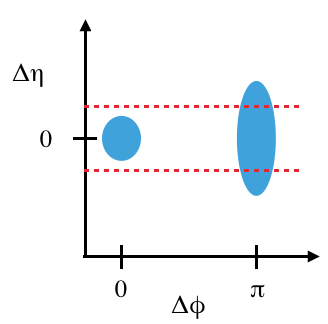
\includegraphics[width=0.5\linewidth]{figs/jet_corr_example.png}
%\caption{TBA}
%\label{fig:jet_corr_example}
%\end{center}
%\end{figure}


%\subsection{Dataset Quality Assurance}
%A PHENIX "run" (lower case r) is defined a group of events that were taken over a single timespan of max length 90 minutes. The for p+Au dataset, there are on 
%average 5 million events per run and there are 339 runs. 
%\begin{figure}[!h]
%\begin{center}
%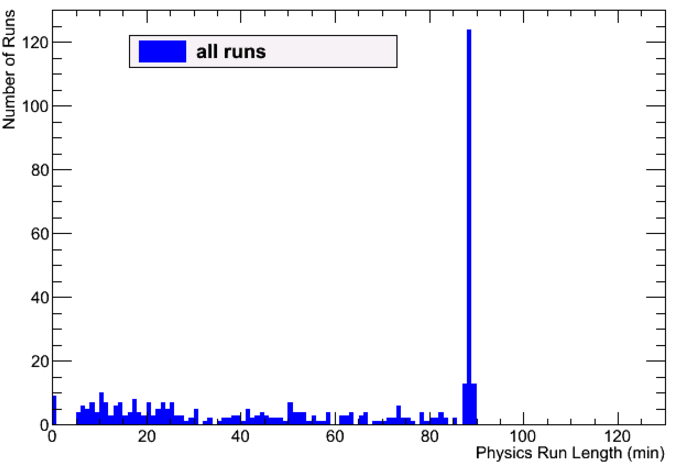
\includegraphics[width=0.65\linewidth]{figs/hruntime.png}
%\caption{The distribution of the length of physics runs.}
%\end{center}
%\end{figure}
%\subsection{luminosity over time}
%RHIC exceeded in delivering its integrated luminosity goals of (\textbf{TO DO: Quantify}).
%\begin{figure}[!h]
%\begin{center}
%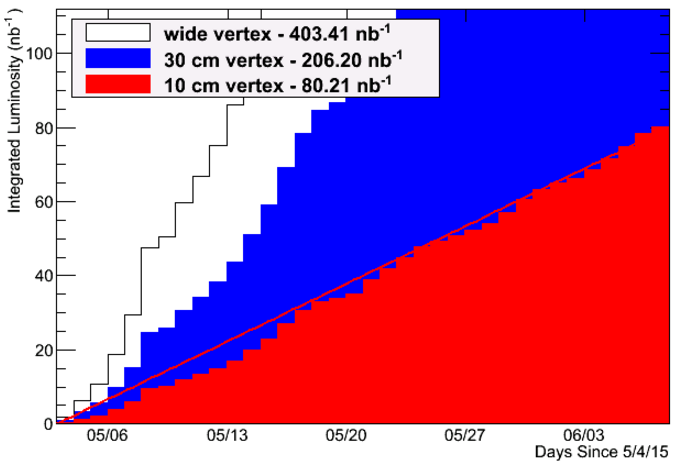
\includegraphics[width=0.65\linewidth]{figs/integrated_luminosity.png}
%\caption{Integrated luminosity from the p+Au dataset.}
%\end{center}
%\end{figure}
%\section{bbc charge}
%\begin{figure}[!h]
%\begin{center}
%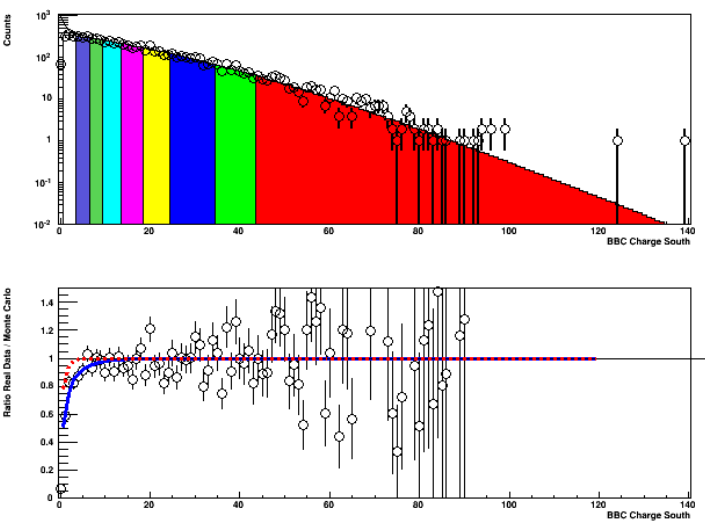
\includegraphics[width=0.65\linewidth]{figs/centrality_determination.png}
%\caption{Real data for BBC Charge South (Au-going direction) shown as open circles and Glauber Monte Carlo + NBD. The colors correspond to the various
%percentiles relative to the total inelastic p+Au cross section, the most central 0-5$\%$ in solid red. The blue and red curves correspond to the Leve-1 trigger
%efficiency in all inelastic collisions and inelastic collisions producing a particle at midrapidity, respectively. The best fit NBD parameters are mu = 3.14, k = 0.47
%, and the trigger firing on 84 +/- 3$\%$ of the total inelastic cross section [sigma = 1.76 barns].}
%\end{center}
%\end{figure}
%\begin{figure}[!h]
%\begin{center}
%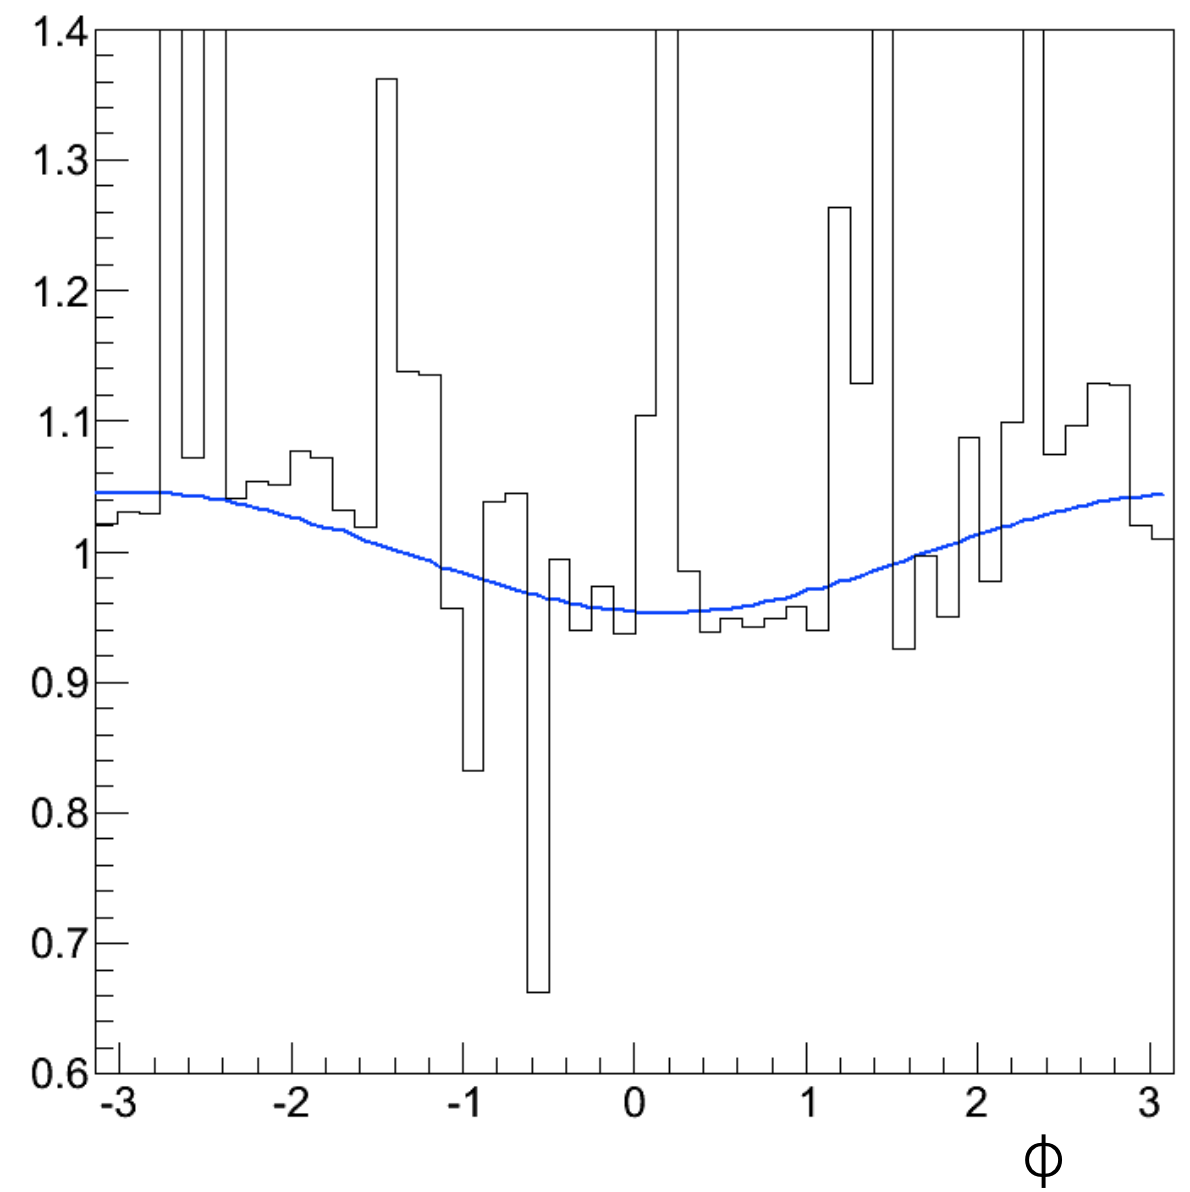
\includegraphics[width=0.5\linewidth]{figs/comparison_of_weights.png}
%\caption{TBA}
%\end{center}
%\end{figure}
%\begin{figure}[!h]
%\begin{center}
%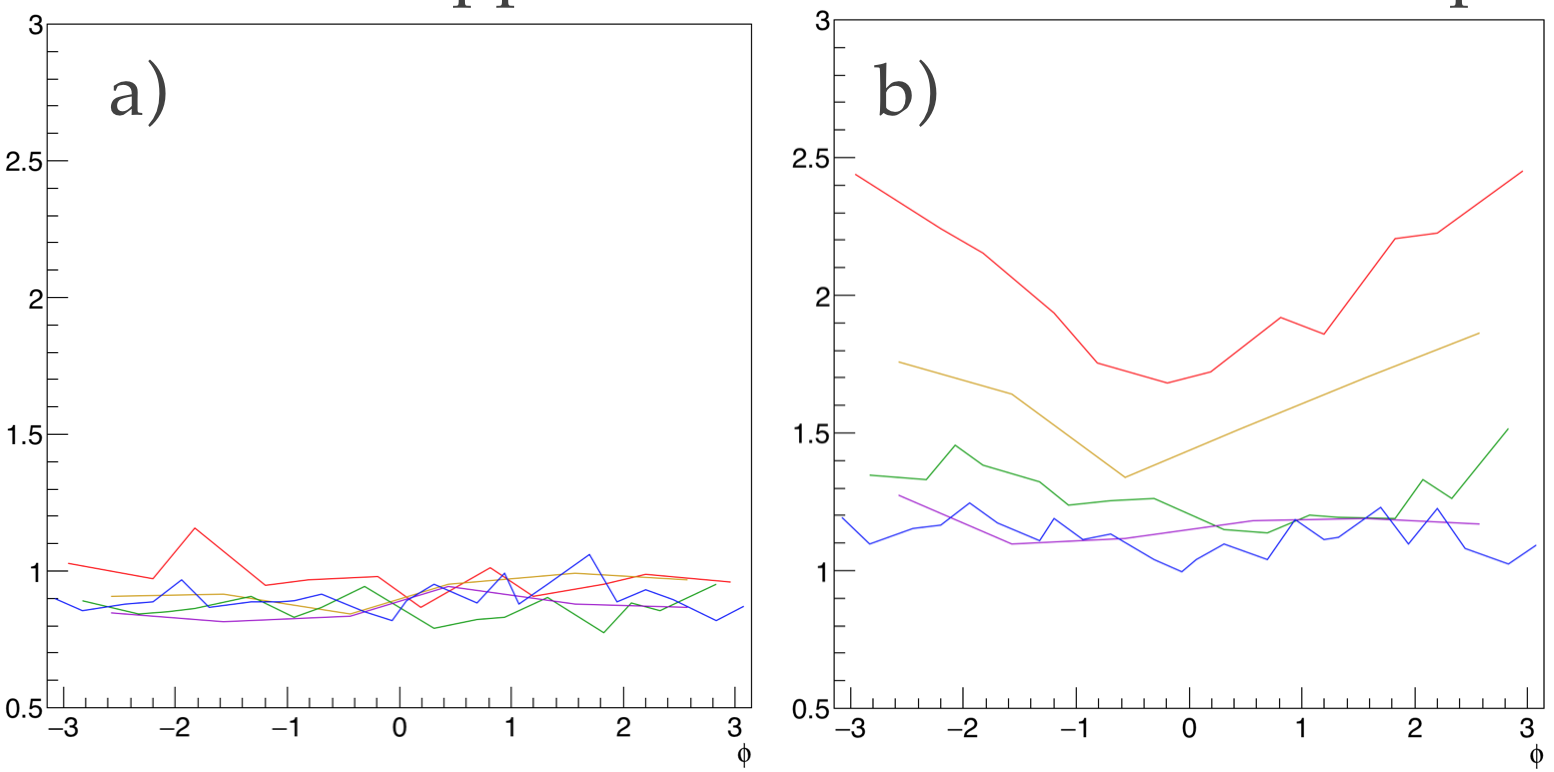
\includegraphics[width=0.6\linewidth]{figs/pp_pau_bbc_comparison.png}
%\caption{These figures show the phi distribution of BBC PMT charge in a) the Run15 pp dataset and in b) the Run15 pAu dataset.}
%\end{center}
%\end{figure}
%\begin{figure}[!h]
%\begin{center}
%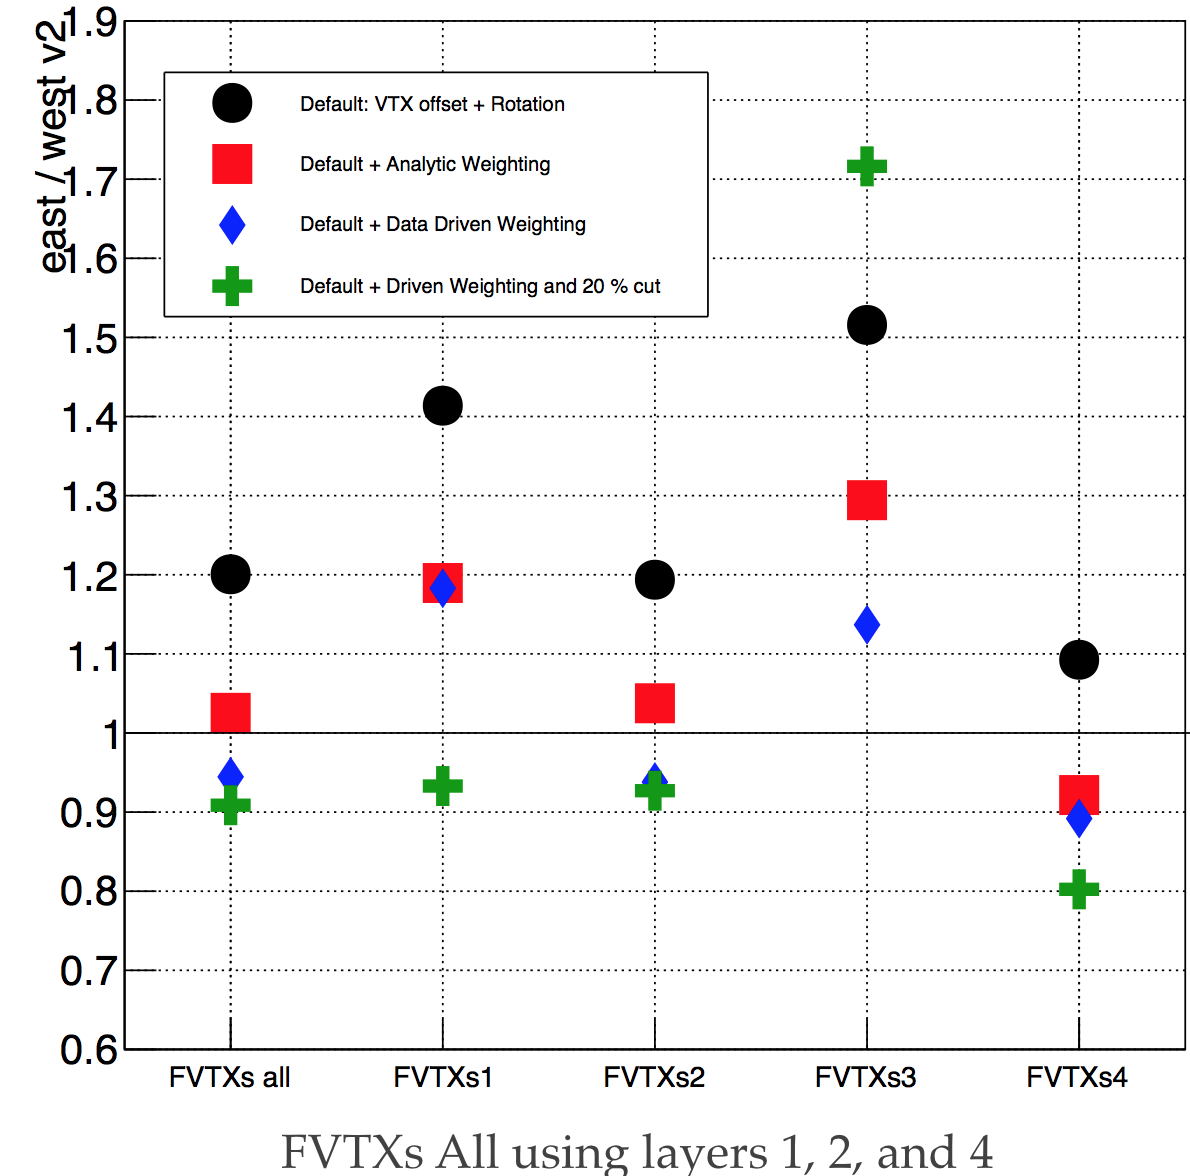
\includegraphics[width=0.5\linewidth]{figs/fvtx_correction_summary.png}
%\caption{TBA}
%\end{center}
%\end{figure}
%\begin{figure}[!h]
%\begin{center}
%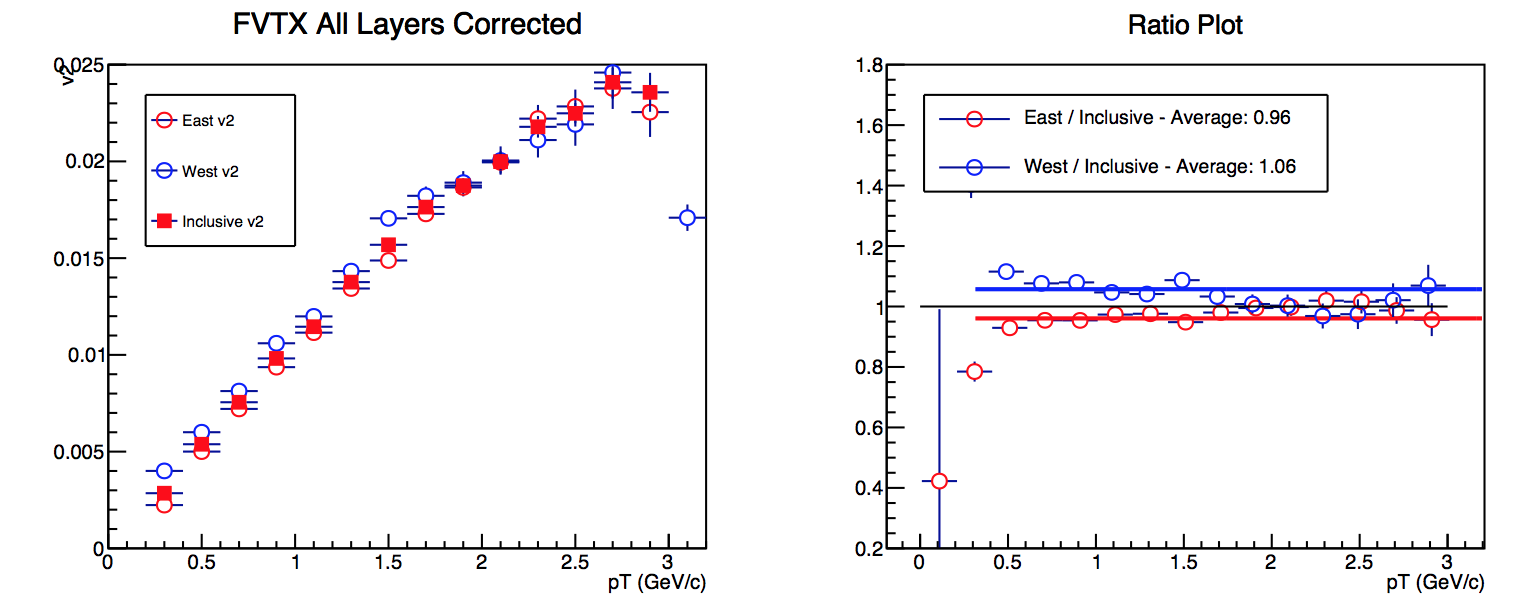
\includegraphics[width=0.5\linewidth]{figs/fvtx_corrected.png}
%\caption{FVTX EP corrected with inverse $\phi$ weighting and 20 $\%$ cut.}
%\end{center}
%\end{figure}
%\begin{figure}[!h]
%\begin{center}
%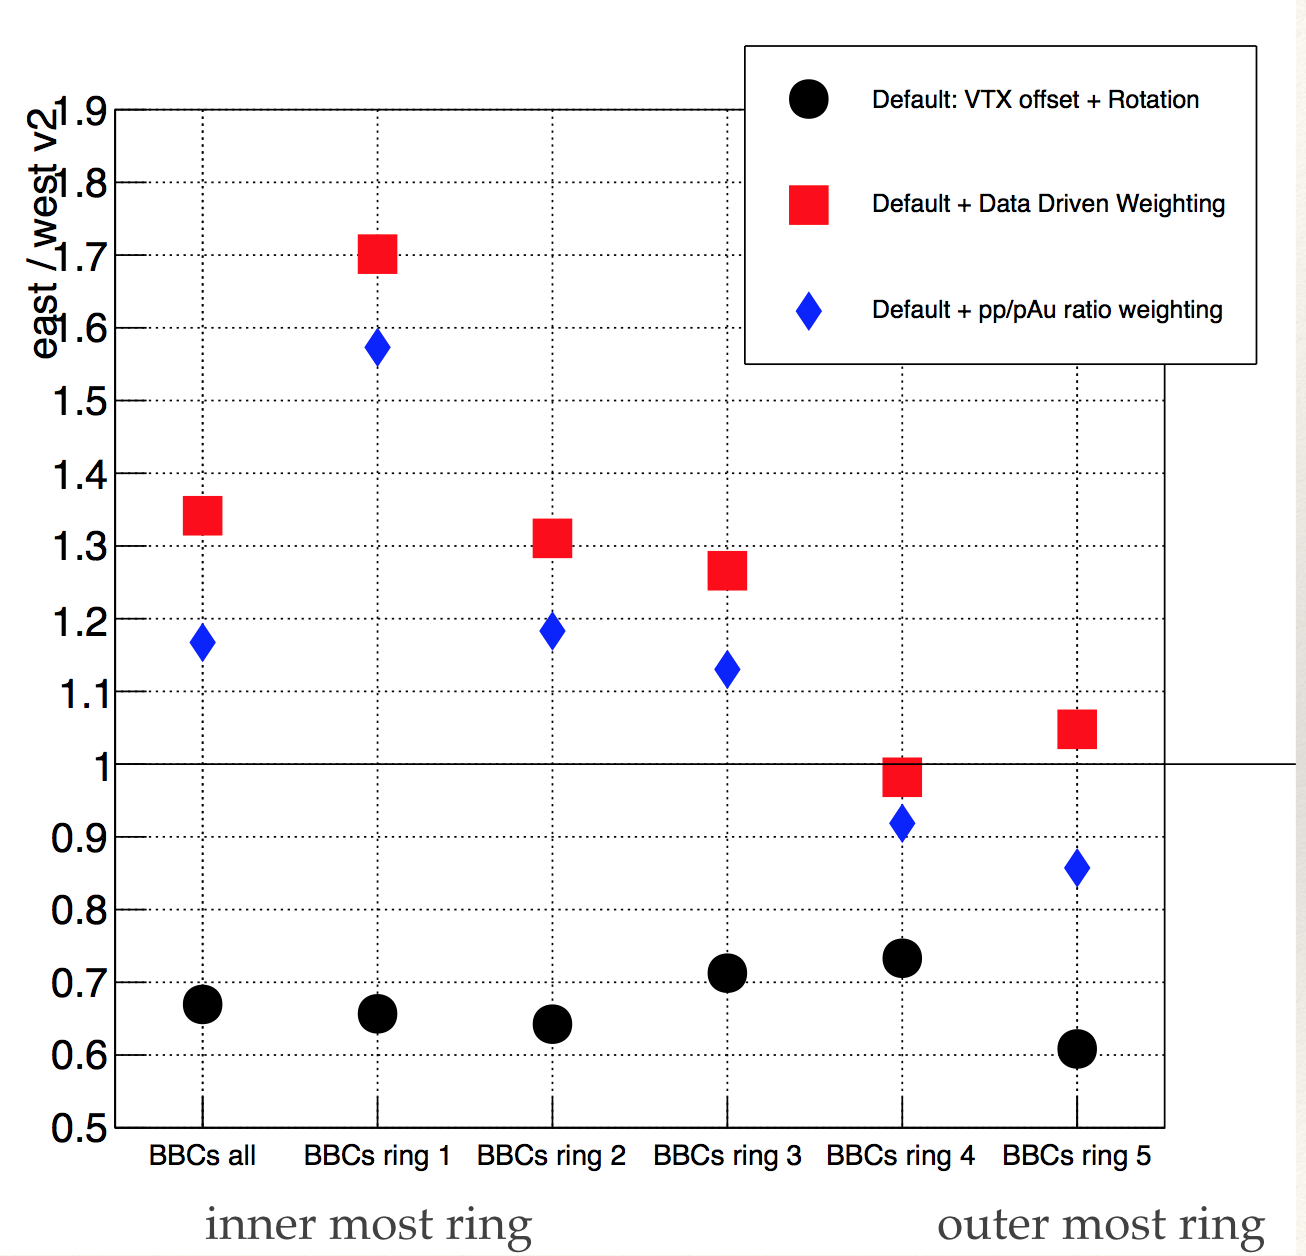
\includegraphics[width=0.5\linewidth]{figs/bbc_correction_summary.png}
%\caption{TBA}
%\end{center}
%\end{figure}
%\begin{figure}[!h]
%\begin{center}
%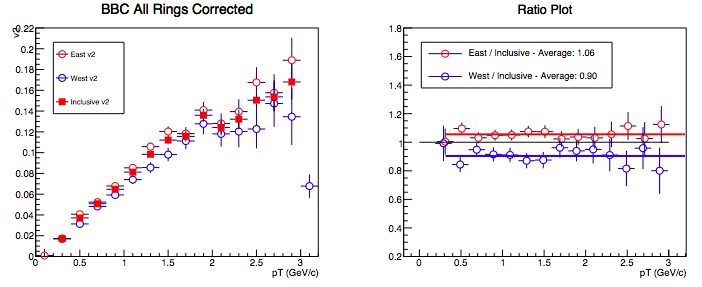
\includegraphics[width=0.5\linewidth]{figs/bbc_pp_correction.png}
%\caption{BBC EP corrected with pp, pau ratio weighting.}
%\end{center}
%\end{figure}
%\begin{figure}[!h]
%\begin{center}
%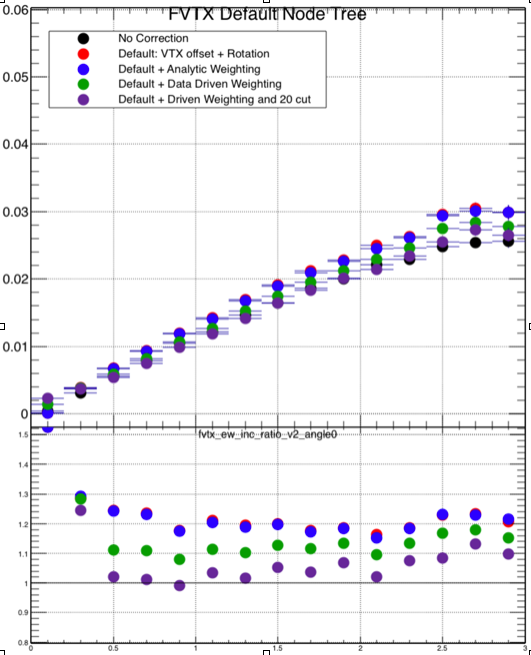
\includegraphics[width=0.5\linewidth]{figs/fvtx_incl_v2_comparison_corrections.png}
%\caption{A comparison of FVTX EP $v_2$ corrections on the inclusive measurement.}
%\end{center}
%\end{figure}
%\section{Systematic Error Estimate}
%\subsection{Non-flow Estimate}
%\begin{figure}[!h]
%\begin{center}
%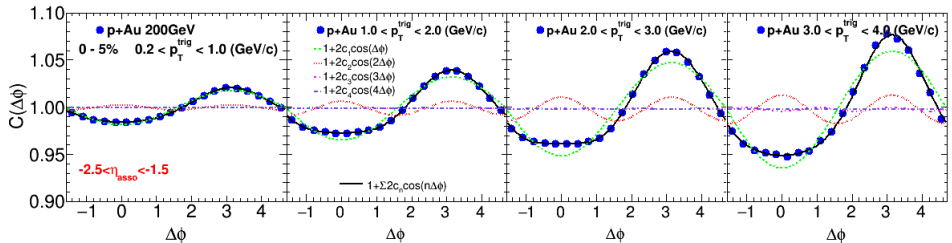
\includegraphics[width=0.6\linewidth]{figs/pau_correlation_central_fvtx.png}
%\caption{TBA}
%\end{center}
%\end{figure}
%\begin{figure}[!h]
%\begin{center}
%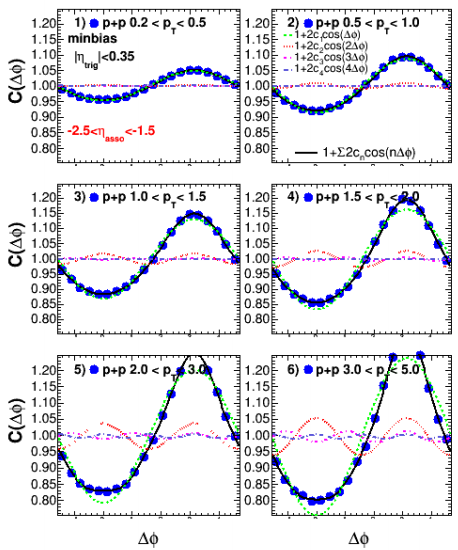
\includegraphics[width=0.6\linewidth]{figs/pp_correlation_minbias_fvtx.png}
%\caption{TBA}
%\end{center}
%\end{figure}
%\begin{figure}[!h]
%\begin{center}
%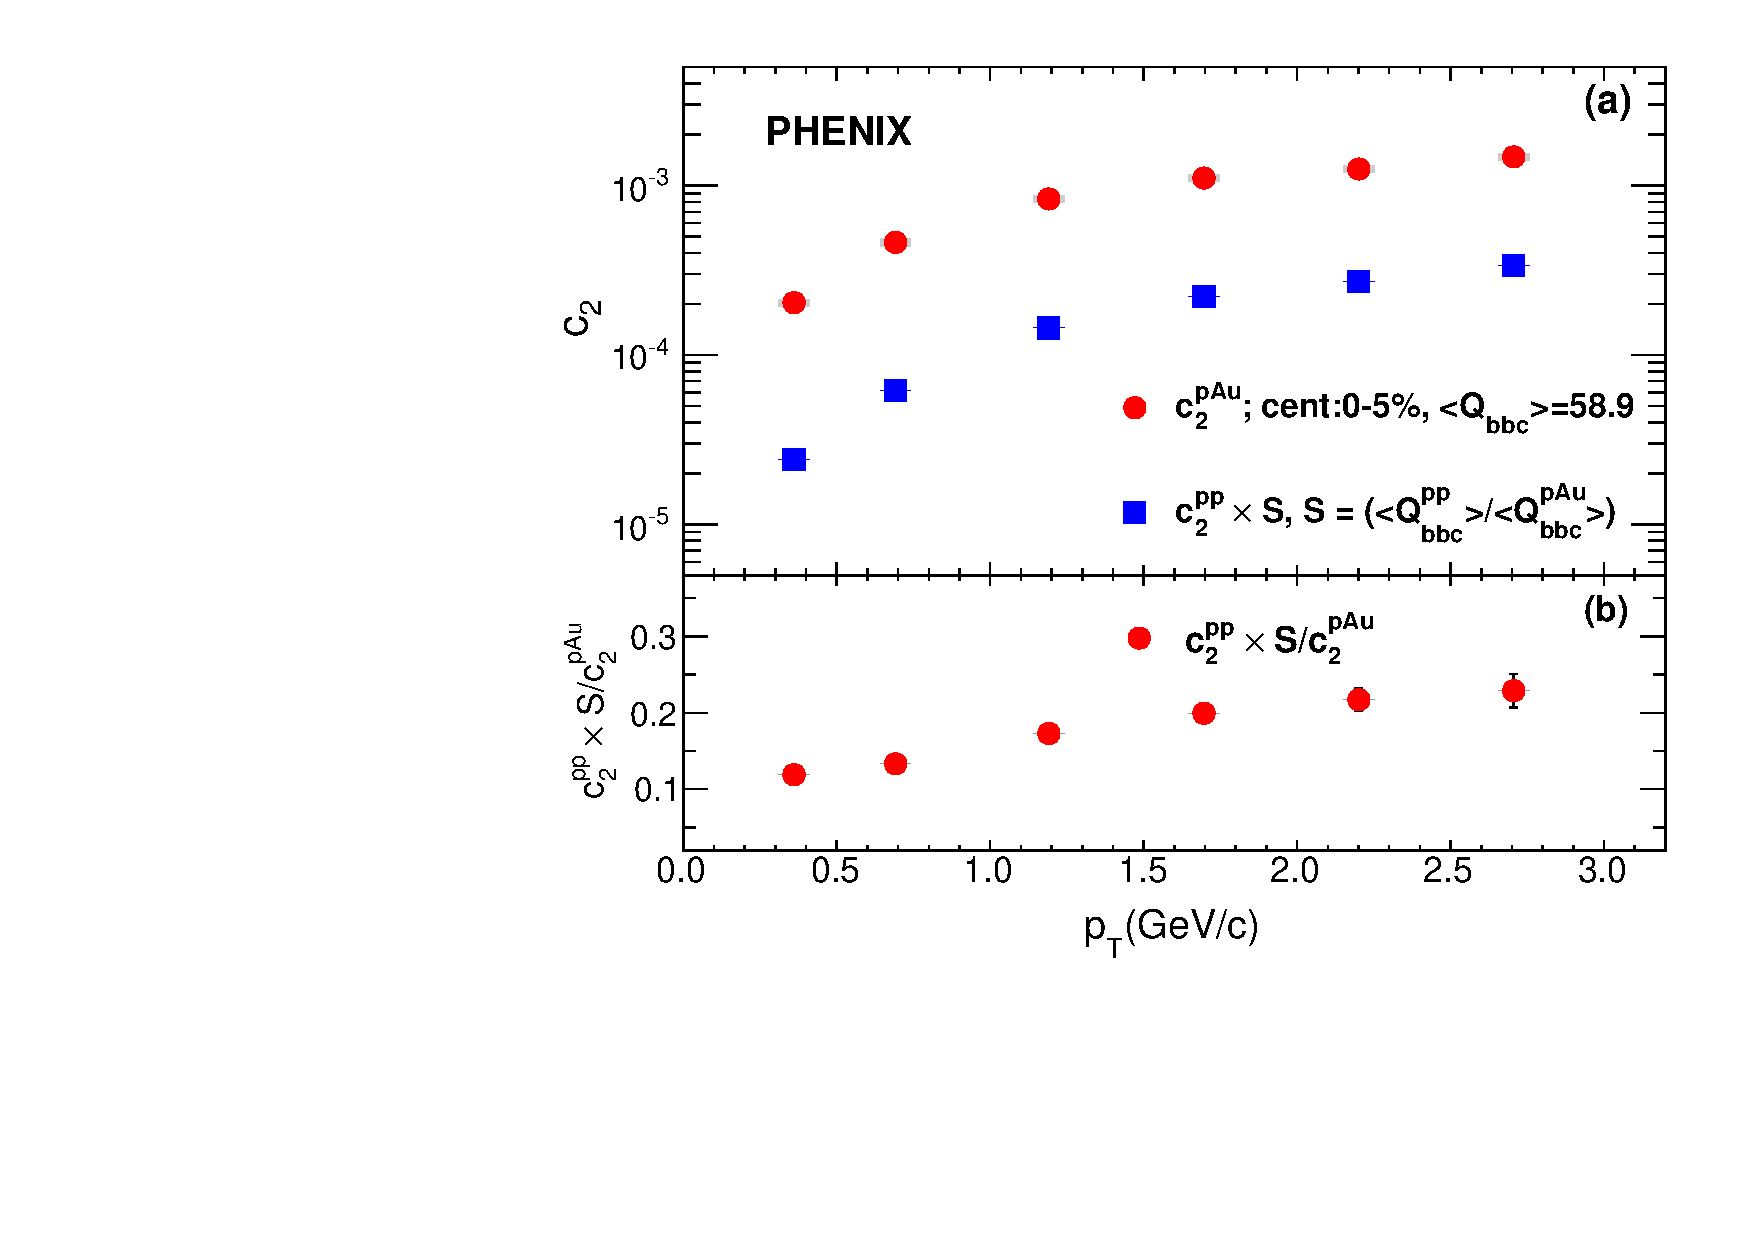
\includegraphics[width=0.6\linewidth]{figs/non_flow.pdf}
%\caption{TBA}
%\end{center}
%\end{figure}
%\subsection{Pile Up}
%\begin{figure}[!h]
%\begin{center}
%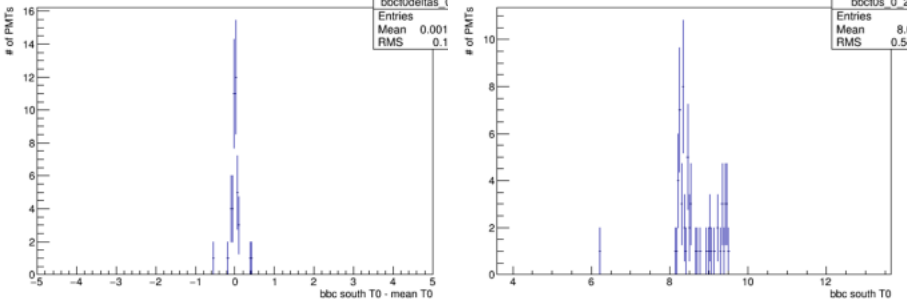
\includegraphics[width=0.6\linewidth]{figs/example_pile_up_event.png}
%\caption{The left plot is an example of a normal event, the right plot is an example pile up event.}
%\end{center}
%\end{figure}
%\subsection{Beam Angle}
%\subsection{Track Background}
%\subsection{Event Plane Detectors Agreement}
